% This is the file main.tex
\usepackage{group4}
\begin{document}
	
	% (The following generates the slides) 
	%---------------------------------------------------------------------------------------------------------------------------------------------------------------------------------------
\mode<presentation>{
	\begin{frame}
	\titlepage
\end{frame}


	\section*{Outline}
	\begin{frame}{Outline}
		\tableofcontents
	\end{frame}
	
\section{Initial Plots}

  
  	\begin{frame}{Second differences with and without seasonal adjustments}
  		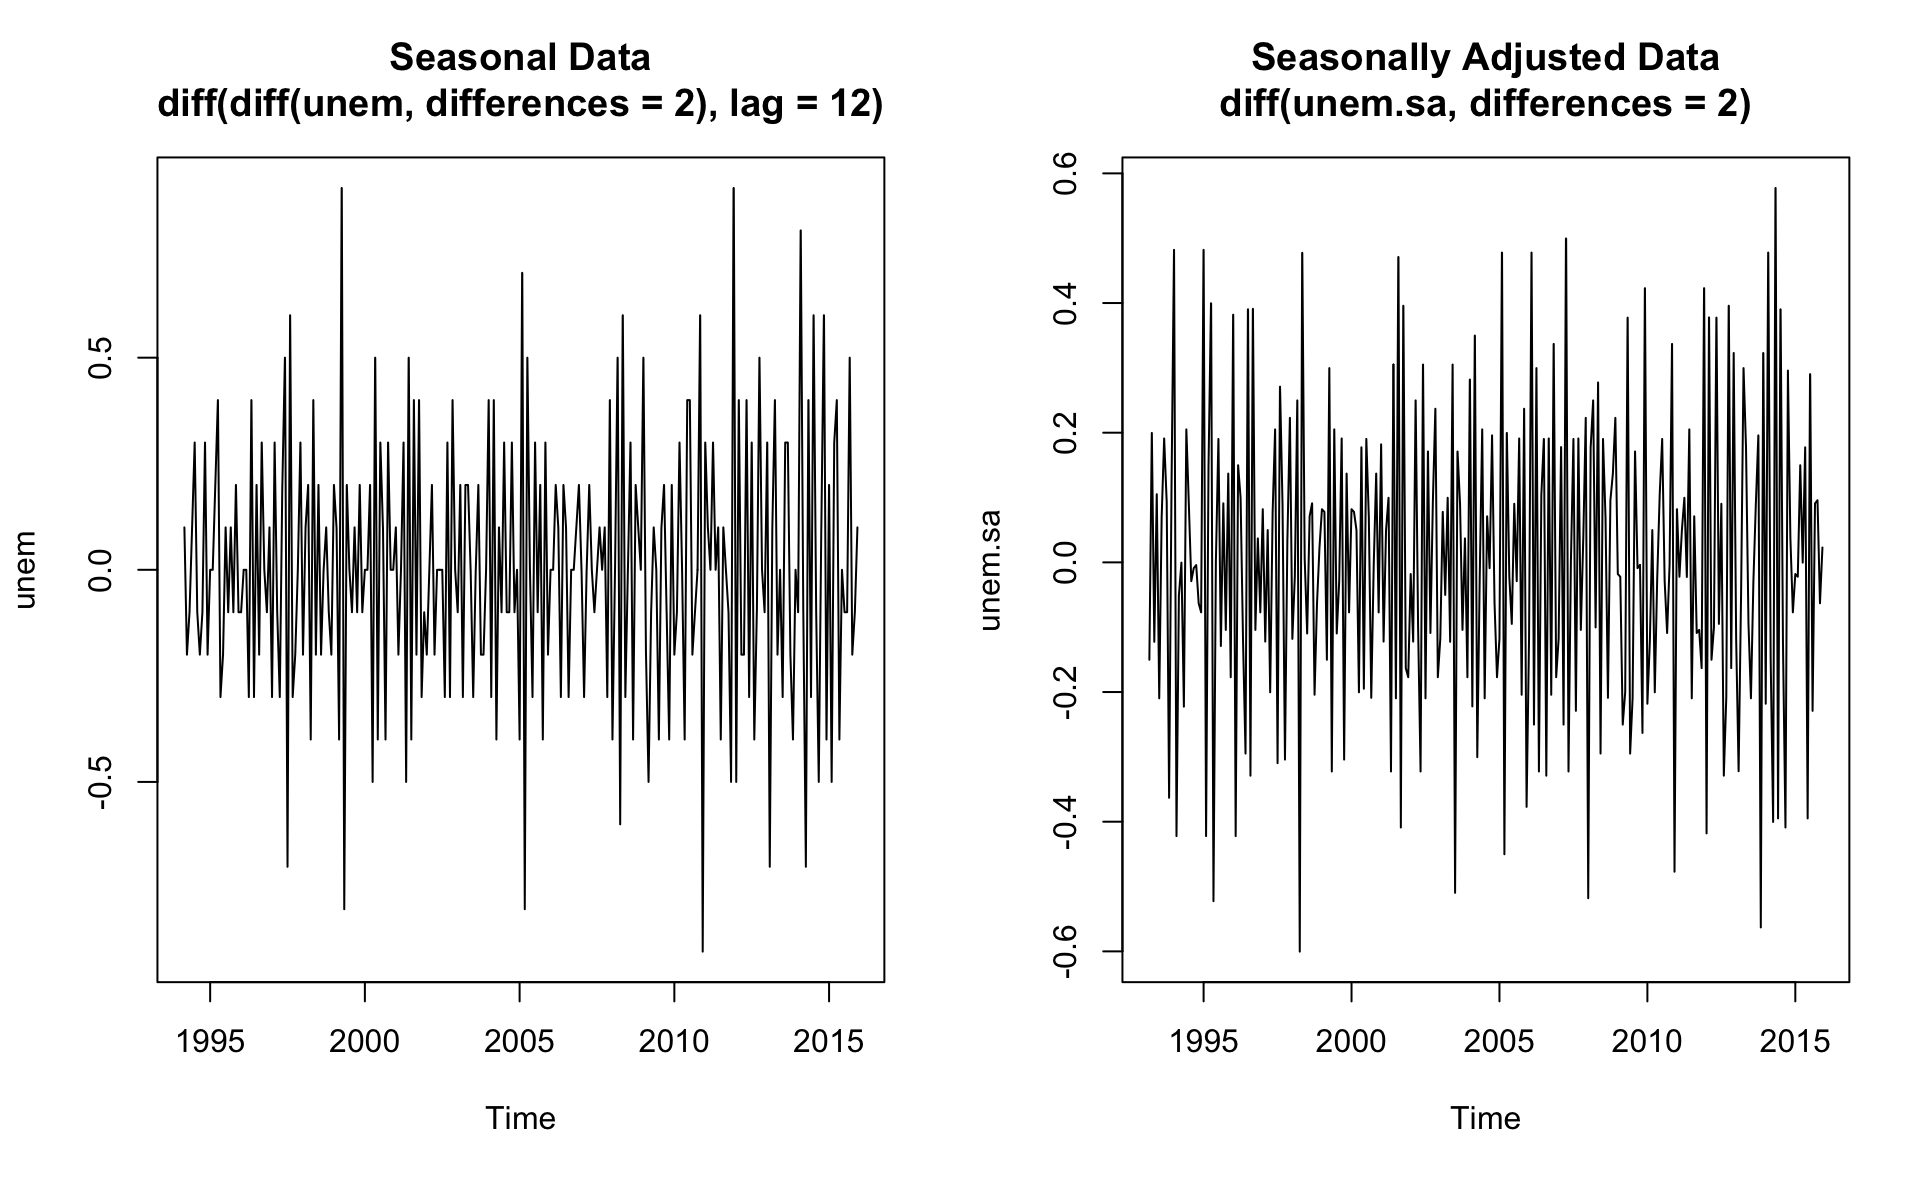
\includegraphics[width=.9\linewidth]{images/stationarity}
  	\end{frame}
  	
  	  
  	  \subsection{ACF \& PACF}
  	  \begin{frame}{ACF \& PACF Plots}
  	  	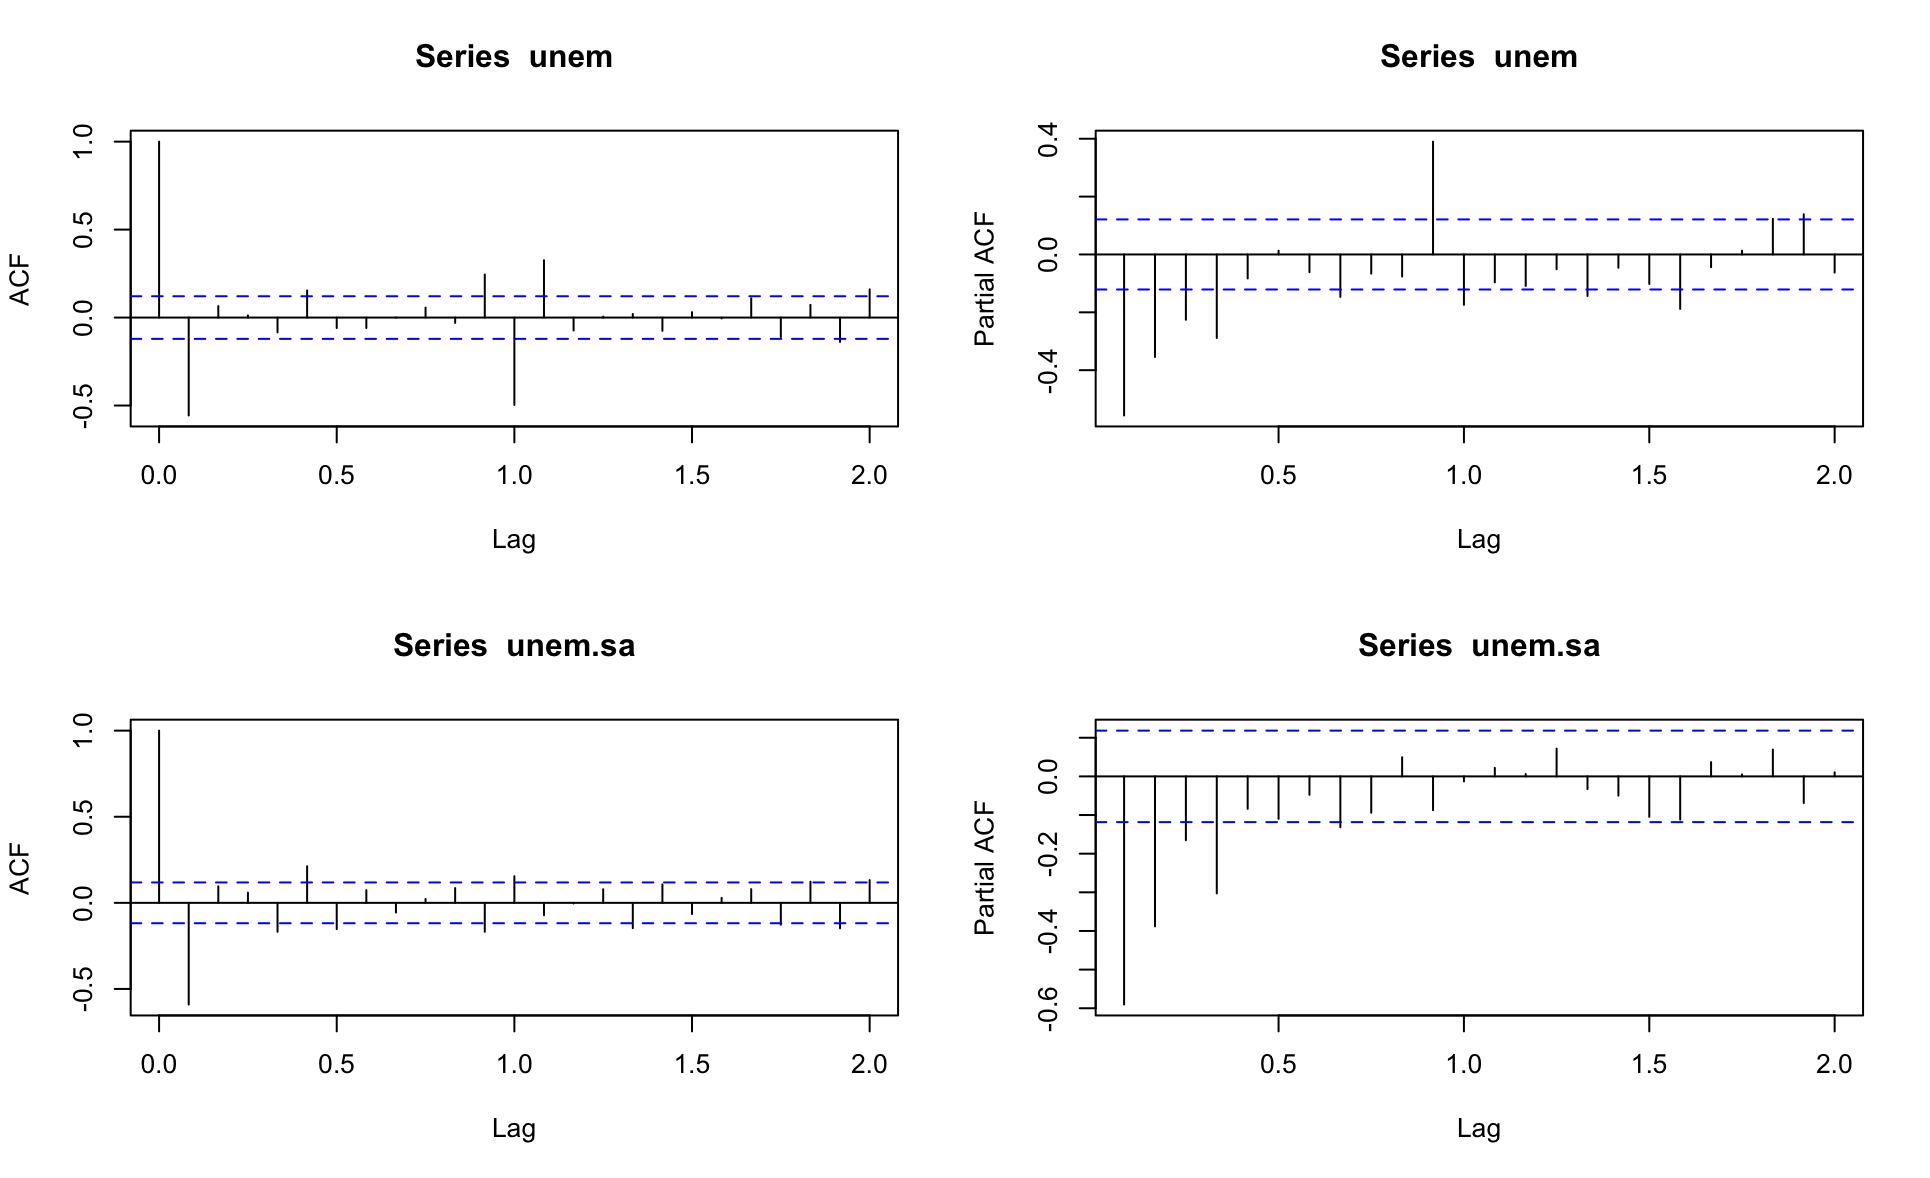
\includegraphics[width=.9\linewidth]{images/acfpacf}
  	  \end{frame}
 
     \subsection{Overview}
     \begin{frame}{Models Considered}
     	% latex table generated in R 3.2.4 by xtable 1.8-2 package
     	% Thu Jul  7 16:13:24 2016
     	\begin{table}[H]
     		\centering
     		\caption{Model Summaries}
     		\begin{tabular}{llccccc}
     			\hline
     			\textbf{\#}& \textbf{Data}  & \textbf{Order} & \textbf{Seasonal} & \textbf{XRegs} & \textbf{AIC} & \textbf{BIC} \\
     			&&&\textbf{Order}&&&\\ 
     			\hline
     			1 & Unem  & 0,2,1 & 1,1,0 & N & -2.27 & -3.23 \\ 
     			2 & Unem  & 0,2,1 & 3,1,0 & N & -2.44 & -3.37 \\ 
     			3 & Unem  & 4,2,1 & 3,1,0 & N & -2.44 & -3.32 \\ 
     			4 & Unem.sa & 0,2,1 & 1,0,0 & N & -2.61 & -3.58 \\ 
     			5 & Unem.sa  & 1,2,1 &  & N & -2.63 & -3.60 \\ 
     			6 & Unem.sa & 0,2,1 & 1,0,0 & Y & -2.58 & -3.49 \\ 
     			7 & Unem.sa  & 1,2,1 &  & Y & -2.60 & -3.49 \\ 
     			\hline
     		\end{tabular}
     		\label{tab:models}
     	\end{table}
     \end{frame}
     %-----------------------------------------------------------------------------------------
     
     \subsection{Seasonal Models}
     %-----------------------------------------------------------------------------------------
     \begin{frame}{Model 1: SARIMA\((0,2,1) \times (1,1,0)_{12}\)}
     	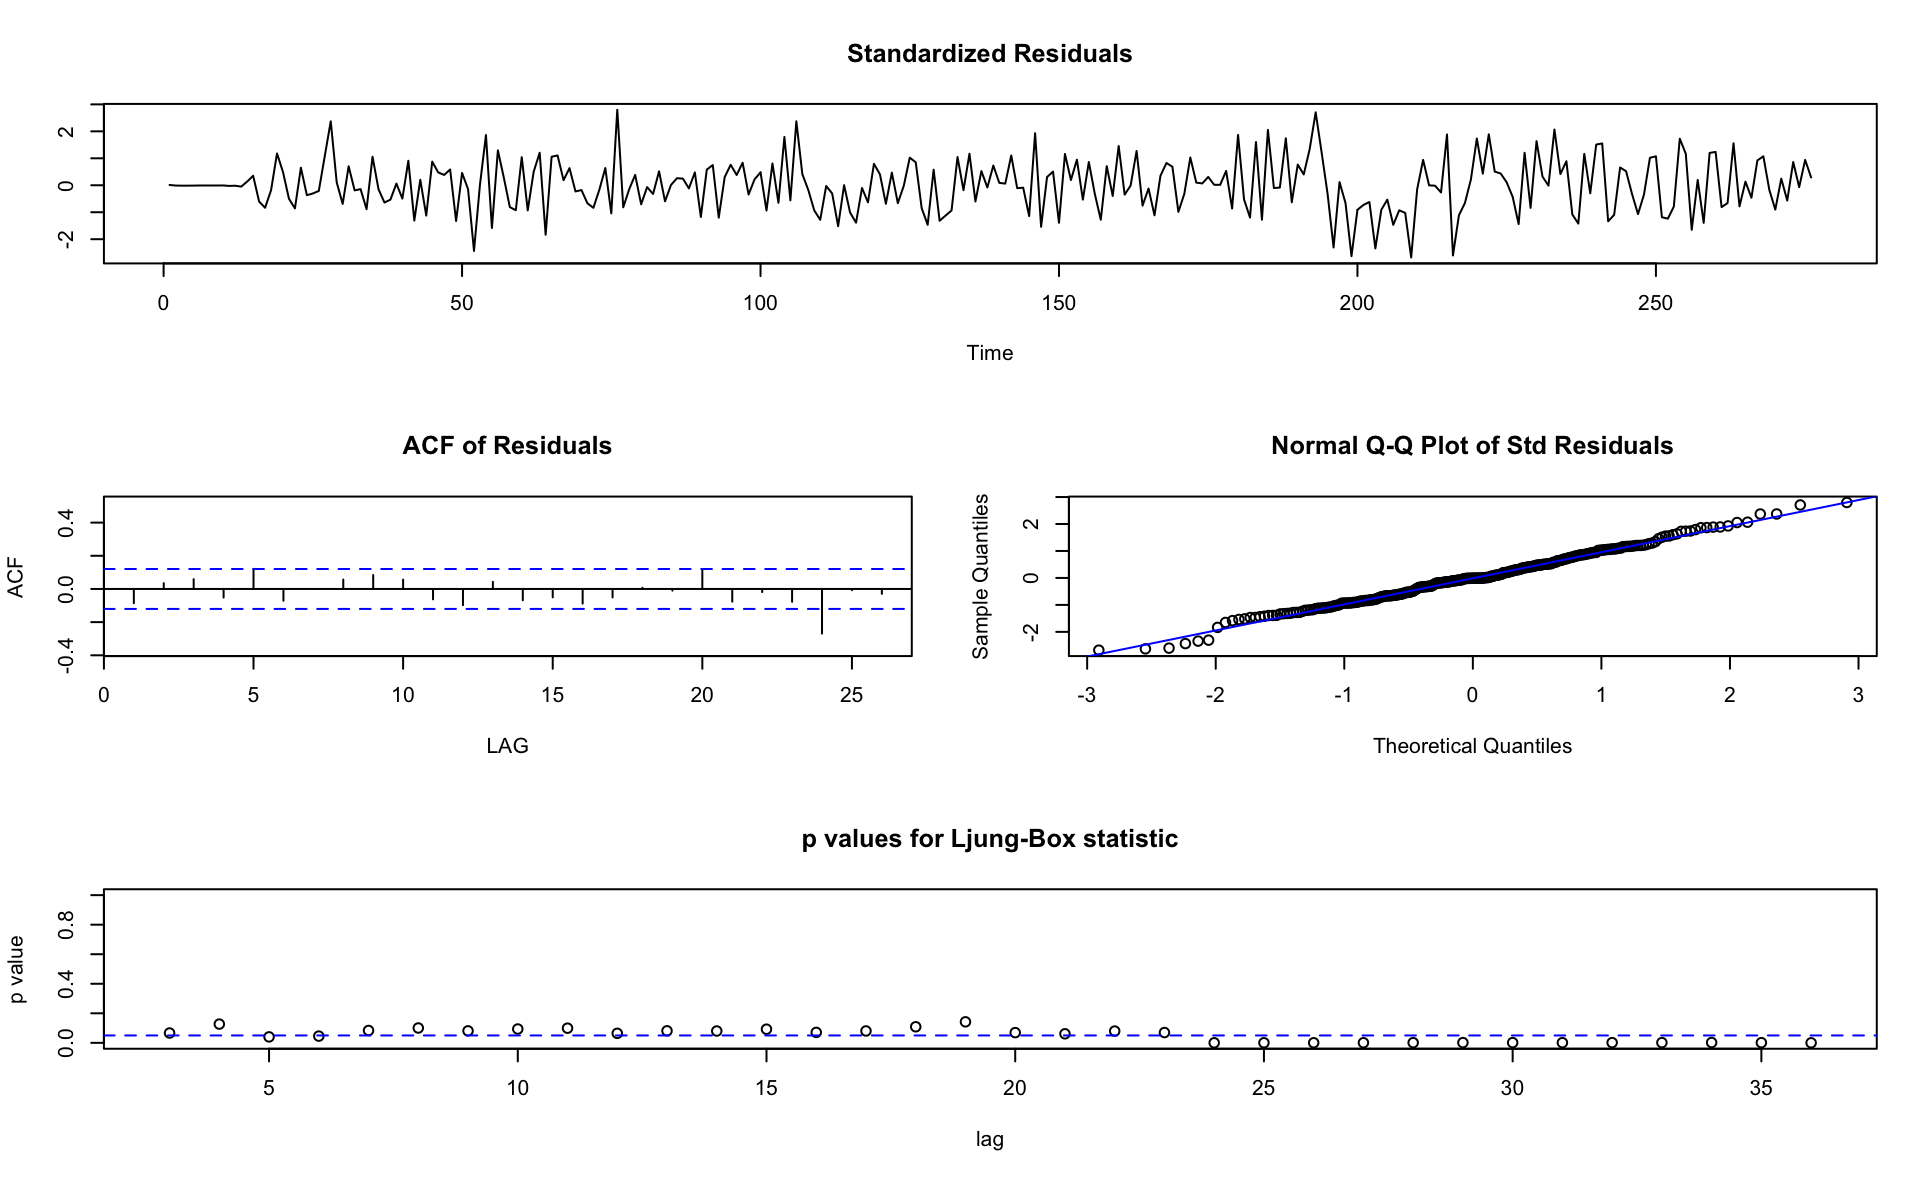
\includegraphics[width=\linewidth]{images/seasonalmodel1}
     \end{frame}
     
     %-----------------------------------------------------------------------------------------
     
     \begin{frame}{Model 2: SARIMA\((0,2,1) \times (3,1,0)_{12}\)}
     	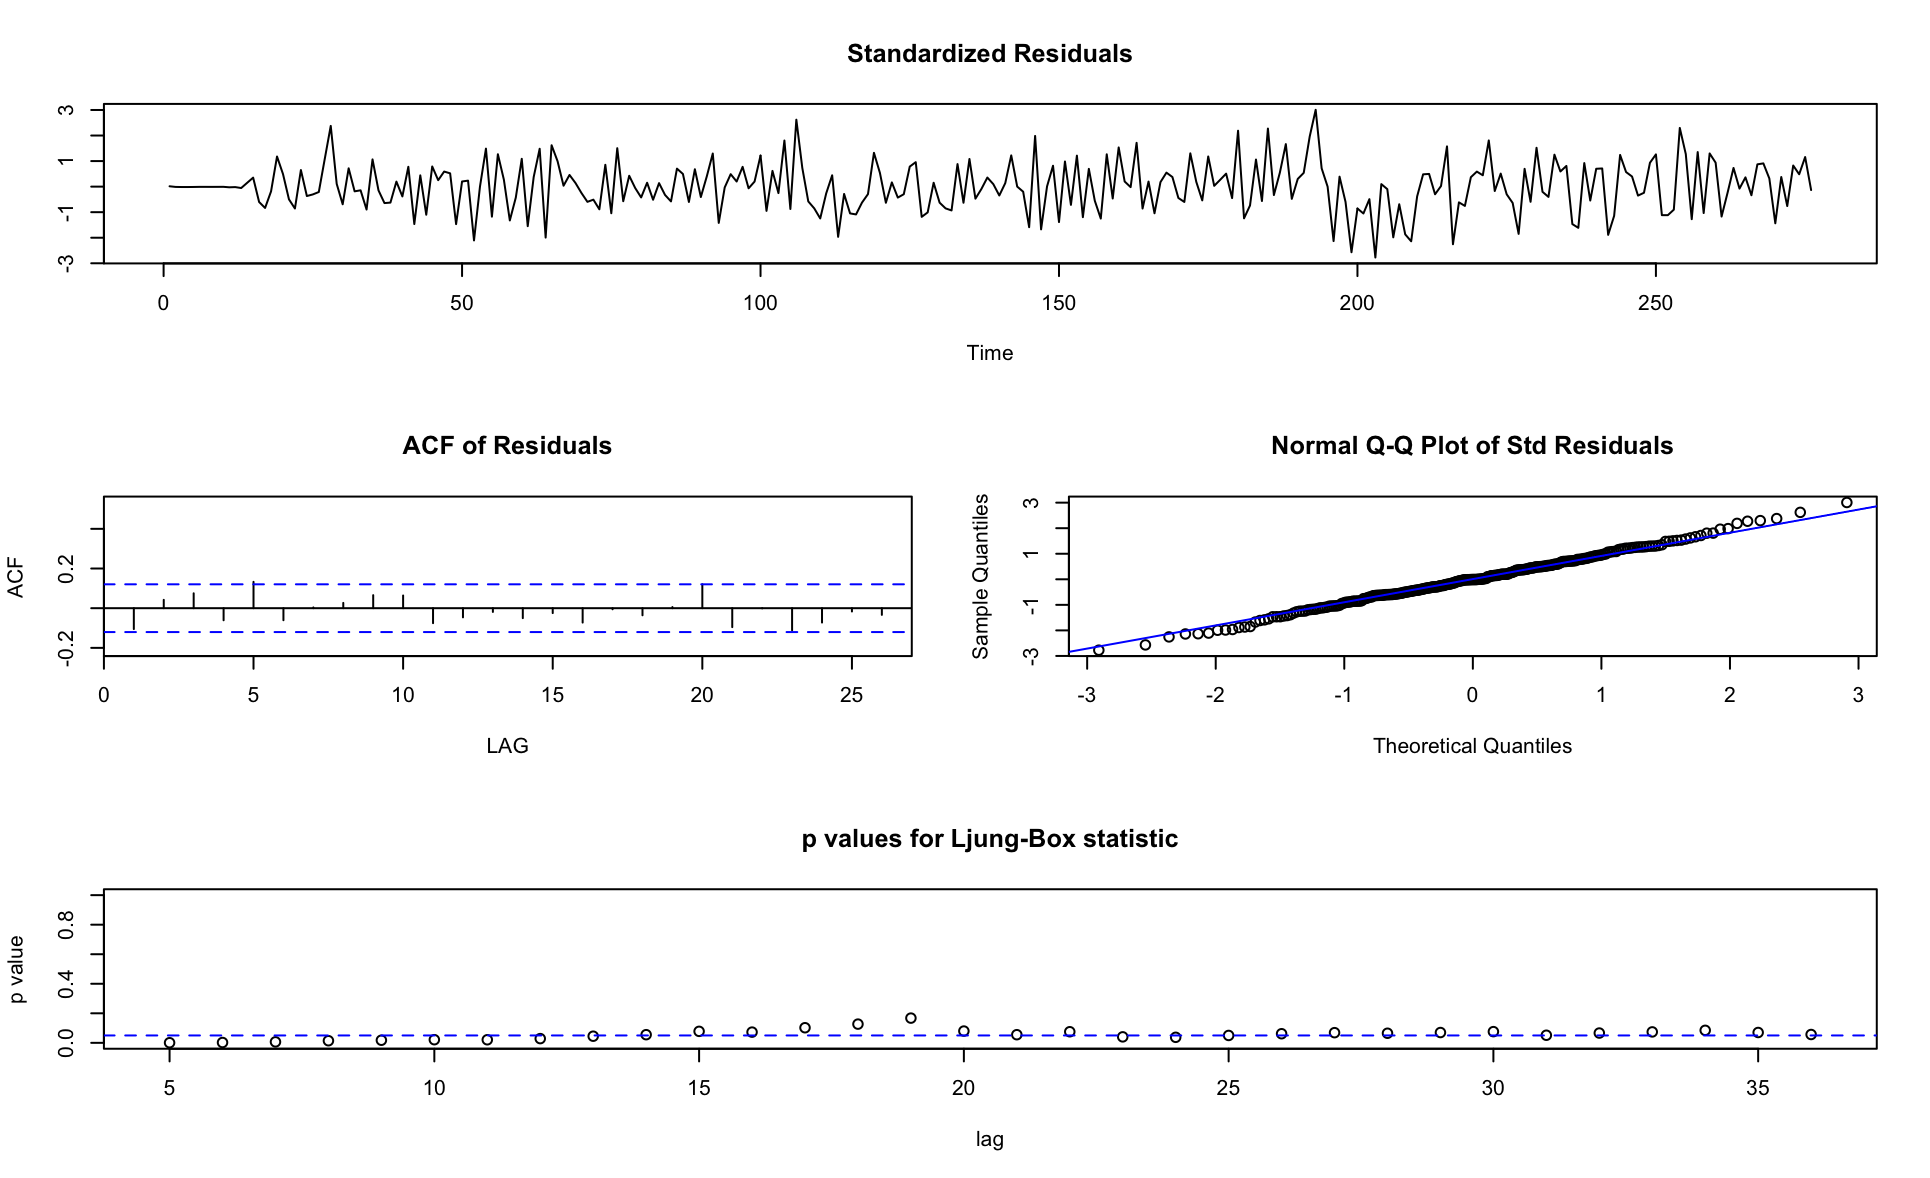
\includegraphics[width=\linewidth]{images/seasonalmodel2}
     \end{frame}  
     
     %-----------------------------------------------------------------------------------------
     
     \begin{frame}{Model 3: SARIMA\((4, 2, 1) \times (3,1,0)_{12}\)}
     	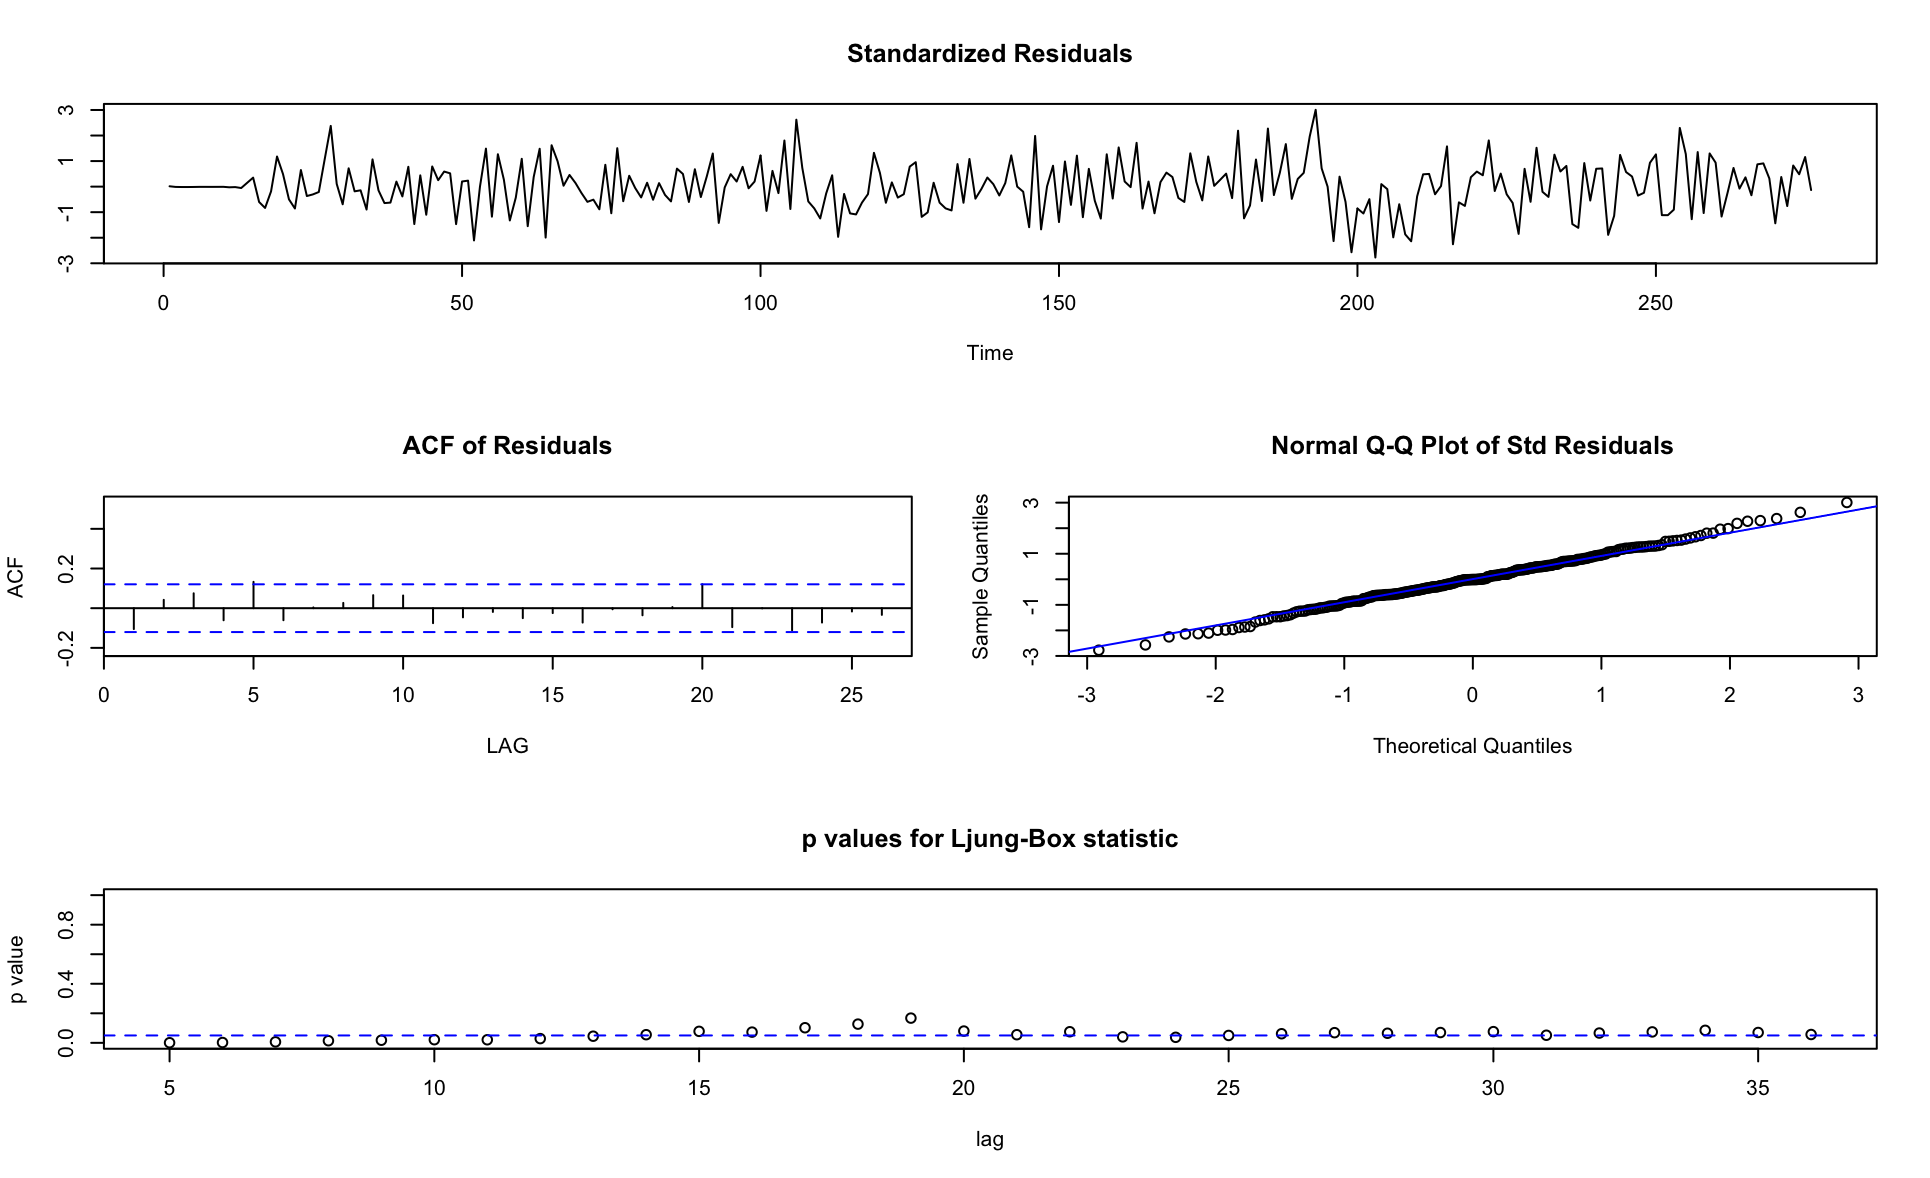
\includegraphics[width=\linewidth]{images/seasonalmodel3}
     \end{frame}  
     %-----------------------------------------------------------------------------------------  
     
     \subsection{Seasonally Adjusted Models}
     %-----------------------------------------------------------------------------------------  
     \begin{frame}{Model 4: SARIMA\((0,2,1) \times (1,0,0)_{12}\)}
     	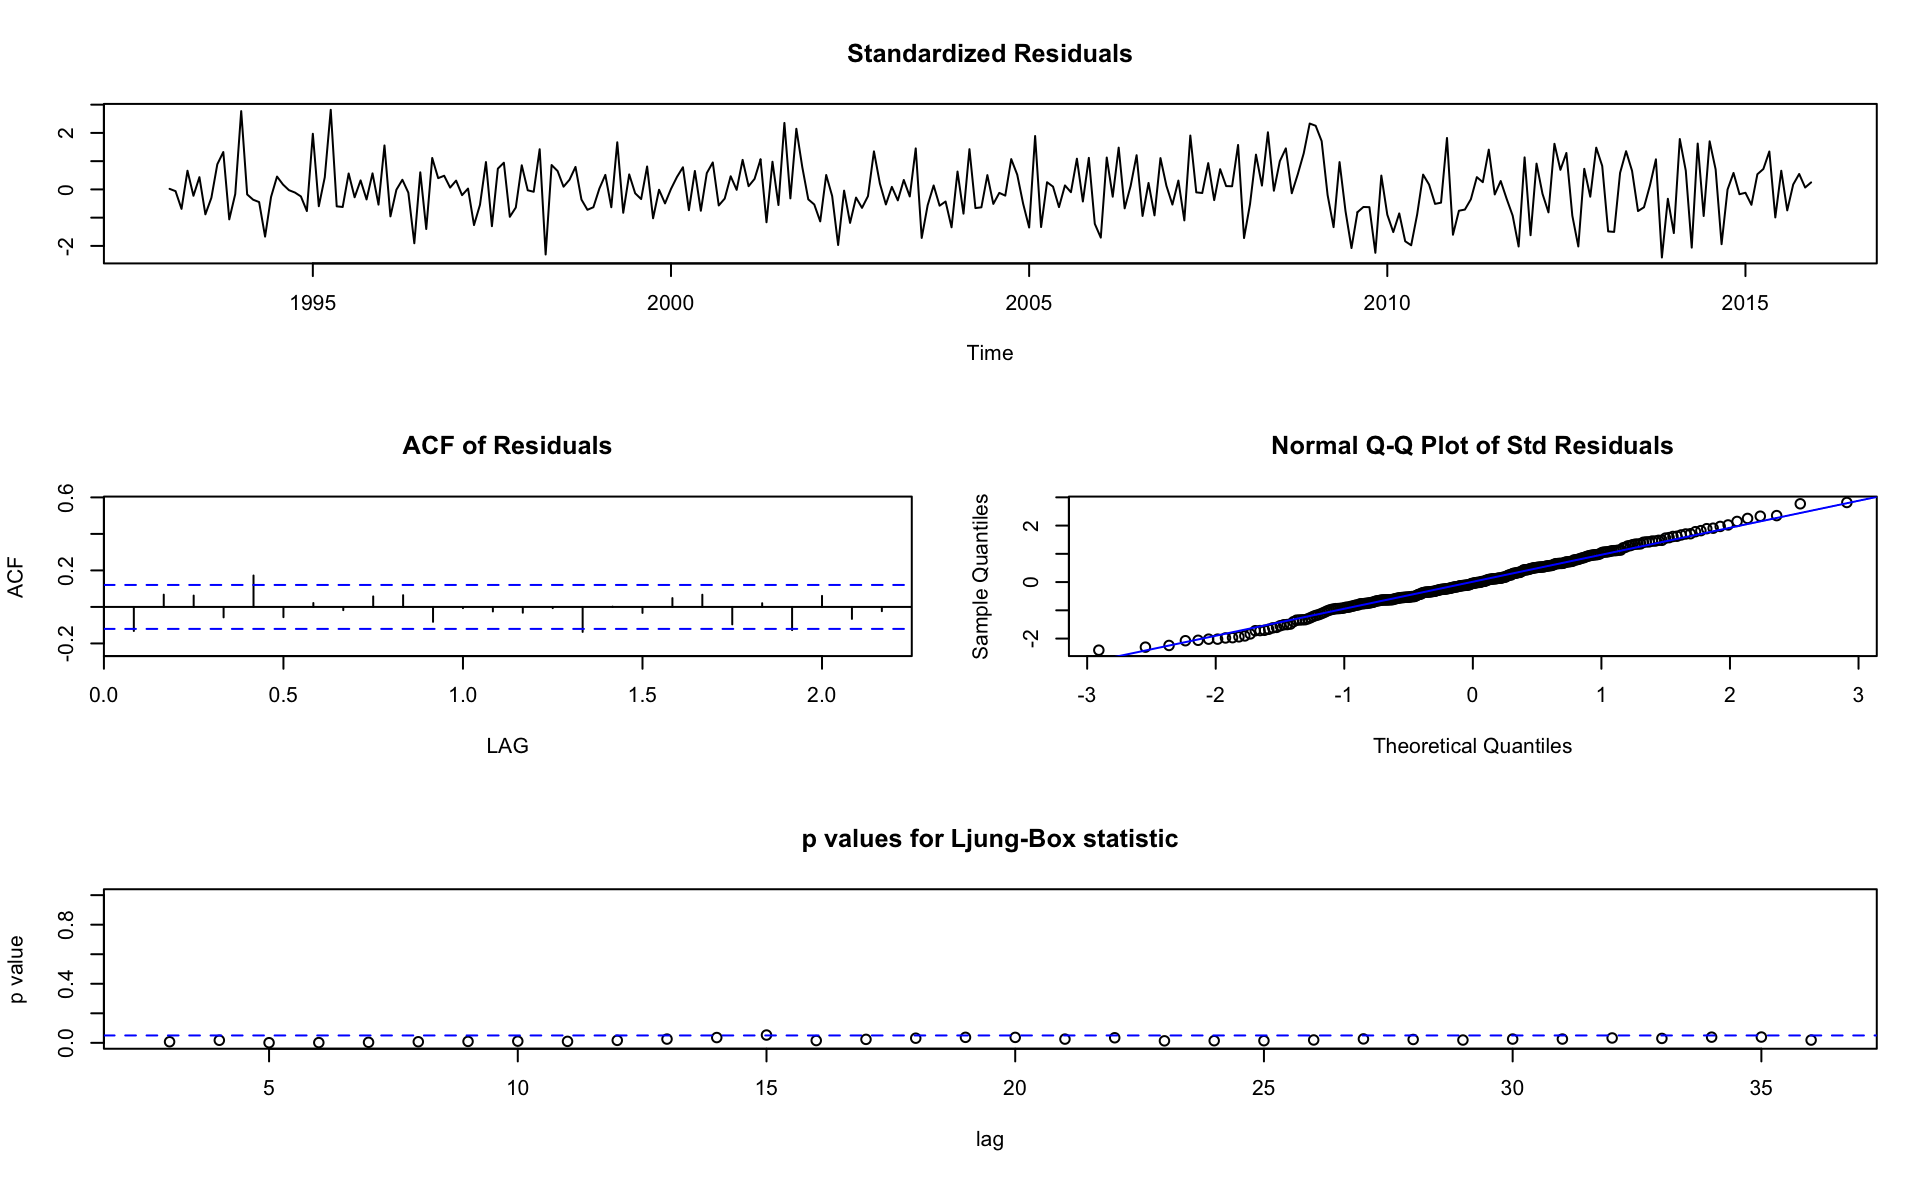
\includegraphics[width=\linewidth]{images/seasonallyadjustedmodel4}
     \end{frame}
     
     %-----------------------------------------------------------------------------------------
     
     \begin{frame}{Model 5: ARIMA\((1,2,1)\)}
     	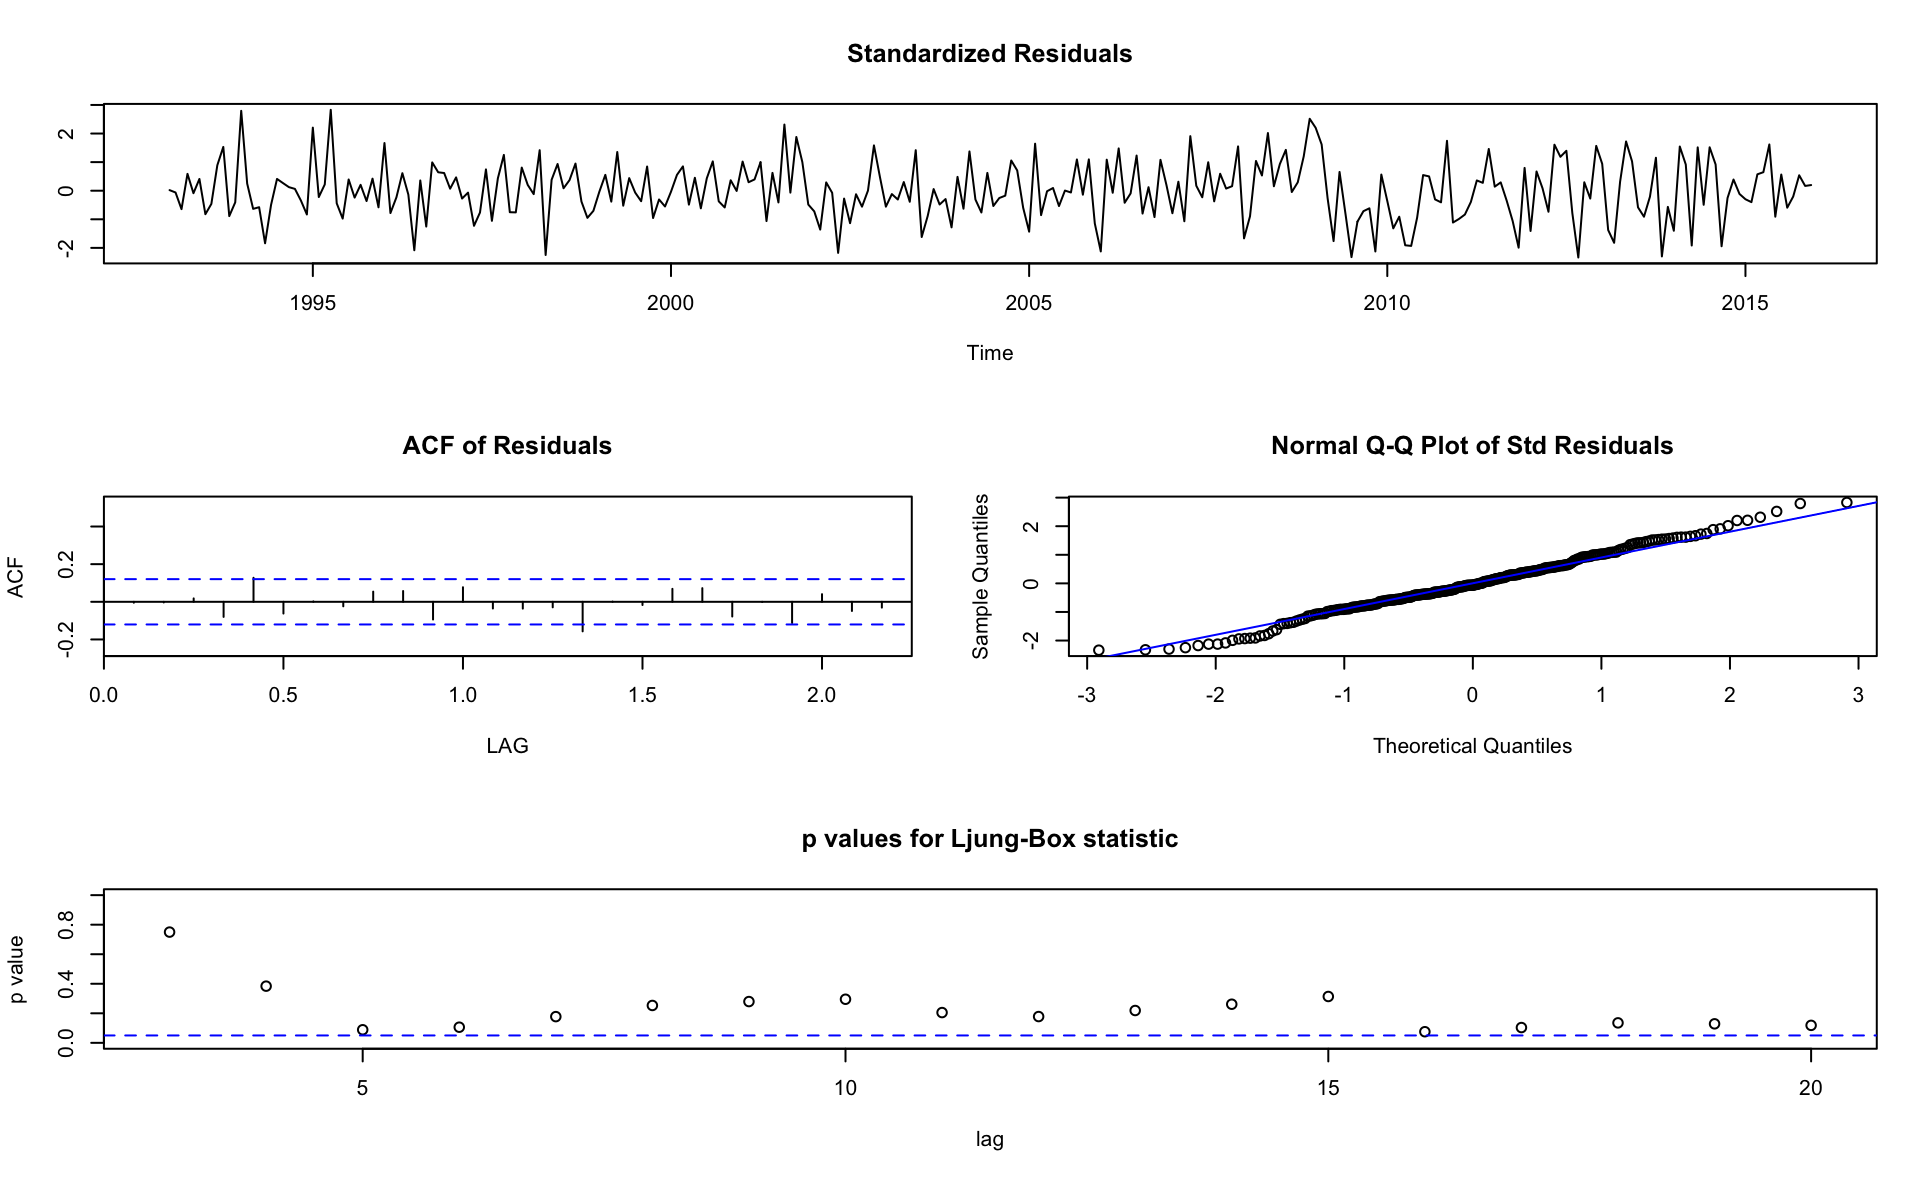
\includegraphics[width=\linewidth]{images/seasonallyadjustedmodel5}
     \end{frame}
     
     %-----------------------------------------------------------------------------------------
     
     \begin{frame}{Model 6: SARIMA\((0,2,1) \times (1,0,0)_{12}\) with Regressors}
     	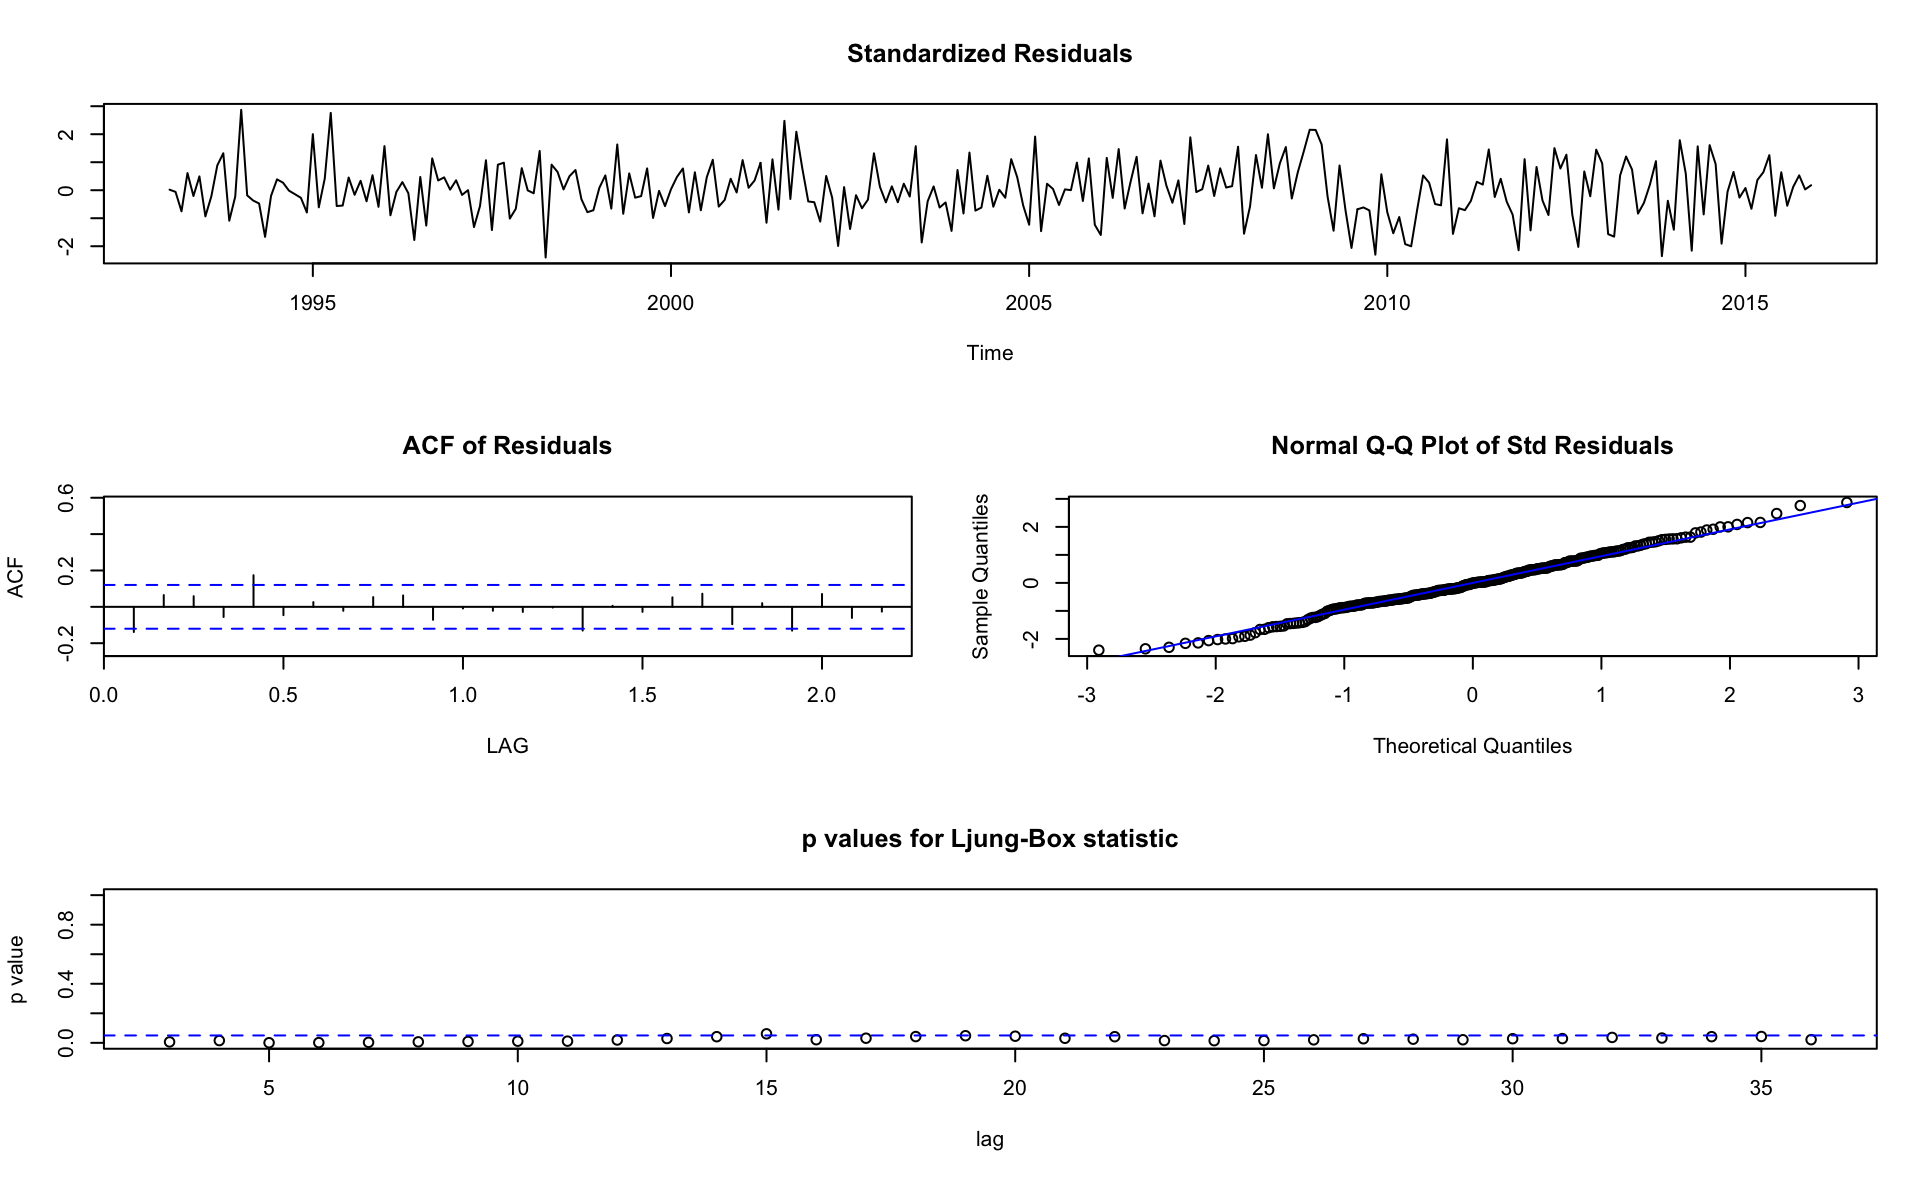
\includegraphics[width=\linewidth]{images/seasonallyadjustedmodel6}
     \end{frame}
     
     %-----------------------------------------------------------------------------------------
     
     \begin{frame}{Model 7: ARIMA\((1,2,1)\) with Regressors}
     	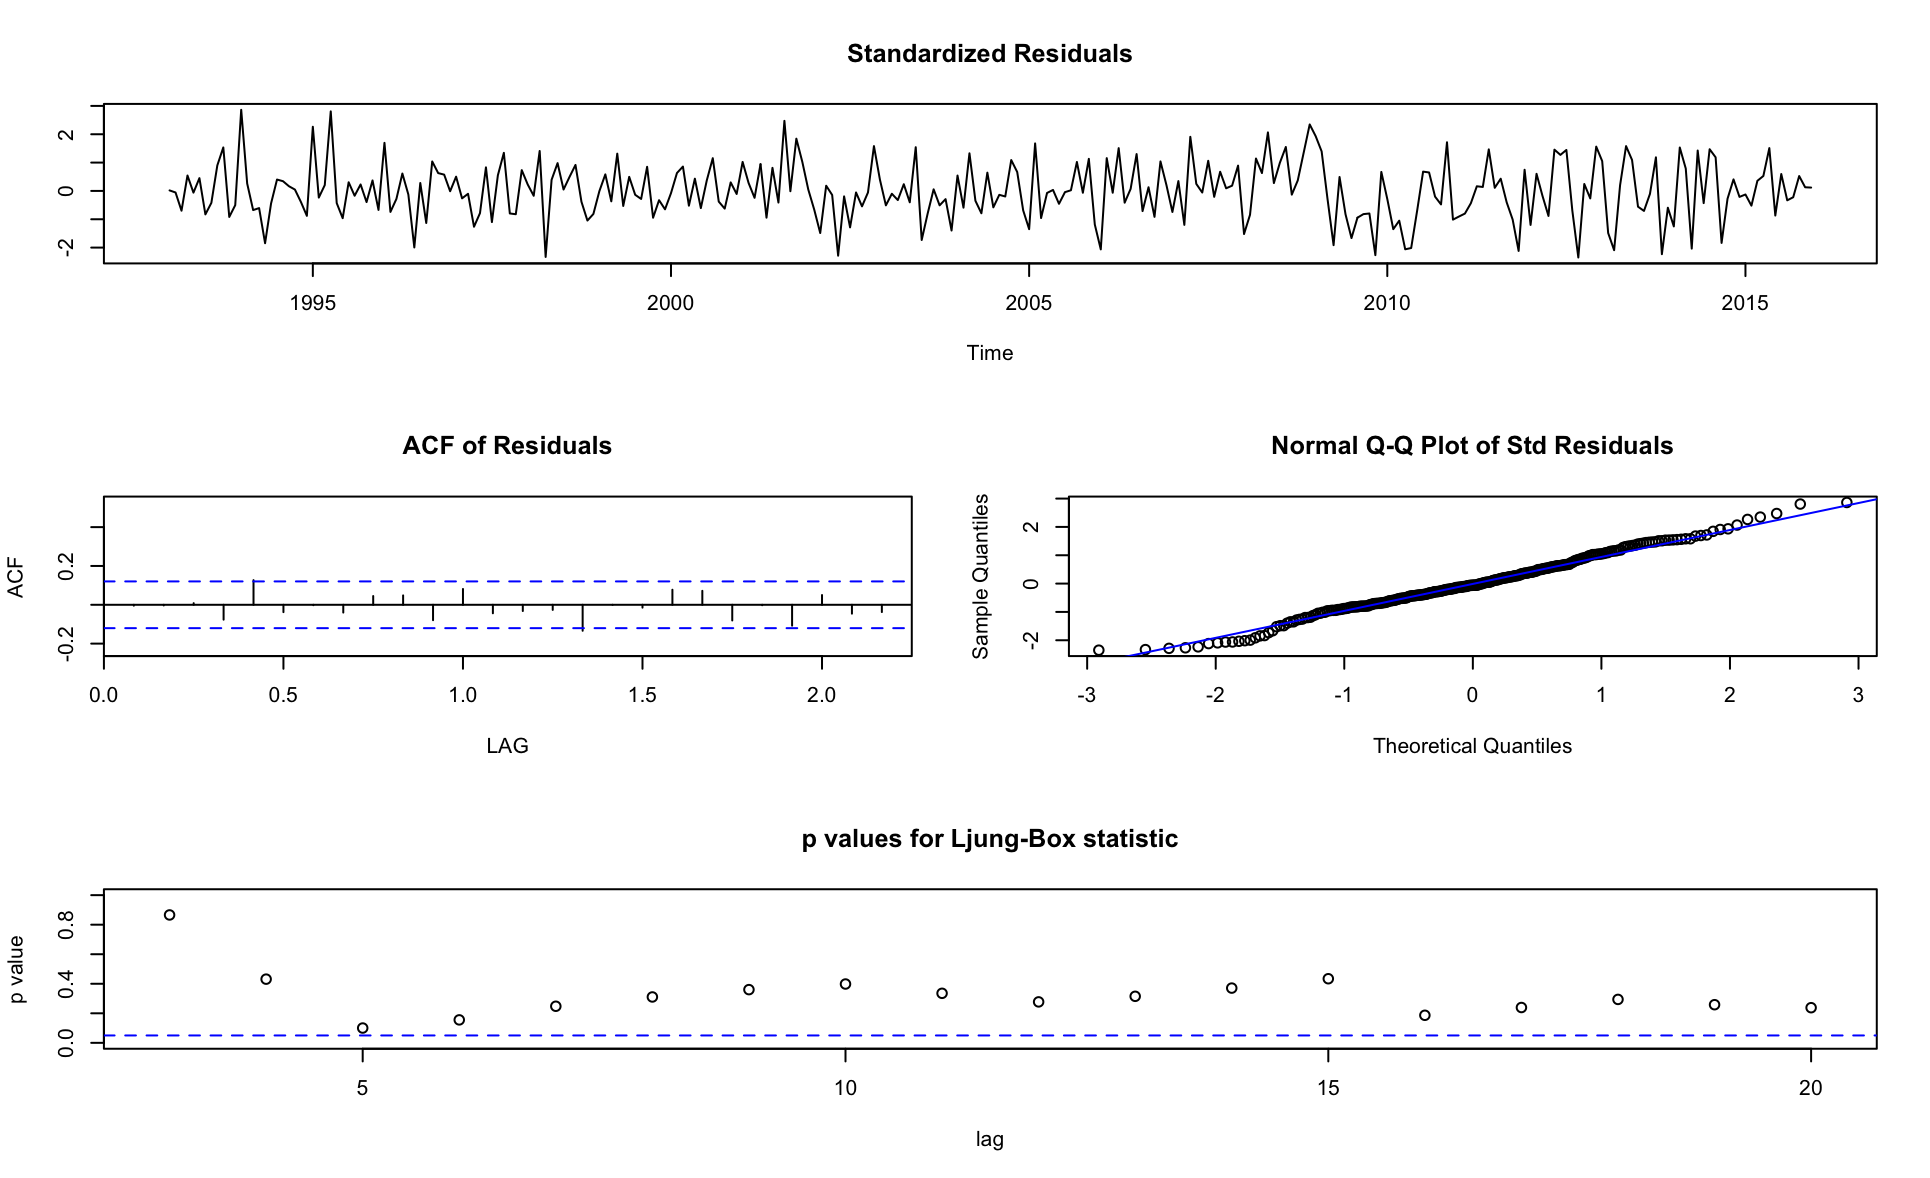
\includegraphics[width=\linewidth]{images/seasonallyadjustedmodel7}
     \end{frame}  
}	
	%--------------------------------------------------------------------------------------------------------------------------------------------------------------------------------------	

% The following generates the write-up
%--------------------------------------------------------------------------------------------------------------------------------------------------------------------------------------	

	
	\mode<article>{
		\title[Unemployment Trends] % (optional, use only with long paper titles)
		{\Huge US Unemployment Trends}
		\subtitle{\huge Initial Model Selection \vspace*{1 cm}}
		\subtitle{\LARGE Group 4}
		
		\date[STAT 626] %(optional, should be abbreviation of conference name)
		{\Large STAT 626: Time Series Analysis}
		% - Either use conference name or its abbreviation.
		% - Not really informative to the audience, more for people (including
		%   yourself) who are reading the slides online
		
		\author[Group 4]{\large Joseph Blubaugh \and Sean Roberson \and Akarshan Puri \and 
			Alison Shelton \and Travis Lilley \and Bo Pang \vspace*{.5 cm}}
		
		\institute[Texas A\&M] % (optional, but mostly needed)
		{Texas A\&M \newline College Station, Texas}
		% - Use the \inst command only if there are several affiliations.
		% - Keep it simple, no one is interested in your street address.

		\pagestyle{fancy}

	\lhead{Group 4}
\chead{}
\rhead{\bfseries US Unemployment Trends} 
\lfoot{}
\cfoot{\thepage}
\rfoot{} 	
		
		\newgeometry{margin=2in}
		\maketitle
		\restoregeometry

		\newpage


		
		
		\subsection*{Introduction}
		
		Unemployment has been a topic of concern throughout the United States in recent years.  Graduate and Undergraduate college students alike are concerned over their employment prospects, wondering if their degrees will be enough to gain them a job after graduation.  In these times of economic uncertainty, obtaining an income generating position is not the guarantee it has seemed to be in generations past. Therefore, the purpose of our project is to examine trends in unemployment in the United States, focusing  on the years from 1992 to 2015, with a goal of forecasting into late 2016 and beyond.  \newline
		
		The unemployment data being examined was obtained from the non-seasonaly adjusted, monthly, Civilian Unemployment Rate Series (UNRATENSA).  In this U.S. Bureau of Labor Statistics (BLS) and included figures from January of 1948 to  May of 2016 \citep{blsref}.  The response variable being analyzed is the unemployment rate defined as the percentage of the labor force that is unemployed.  In defining this variable, the BLS restricts this to, ``people 16 years of age and older, who currently reside in 1 of the 50 states or the District of Columbia, who do not reside in institutions (e.g., penal and mental facilities, homes for the aged), and who are not on active duty in the Armed Forces''. \newline
		
		As a first step, the data was plotted over time to identify any obvious patterns visually, considering both seasonlly adjusted and non-seasonlly adjusted versions of the unemployment rate, See Figure \ref{fig:unemployment}.  The time span included in the study encompases the presidential terms of Bill Clinton, George W. Bush, and Barack Obama, each serving eight years in office.  Initial graphs of the data seem to indicate that, in general, unemployment spiked at the begining of each president's term and fell gradually over the time he was in office. There are also two noticeable spikes the represent that recessions of 2001 and 2008, respectively.  The 2008 recession also follows the burst of a housing market bubble.  These are all potential explanatory variables that will be explored in further analysis.
		\begin{figure}[H]
			\centering
			\caption{Plot of the original data}
			\label{fig:unemployment}
			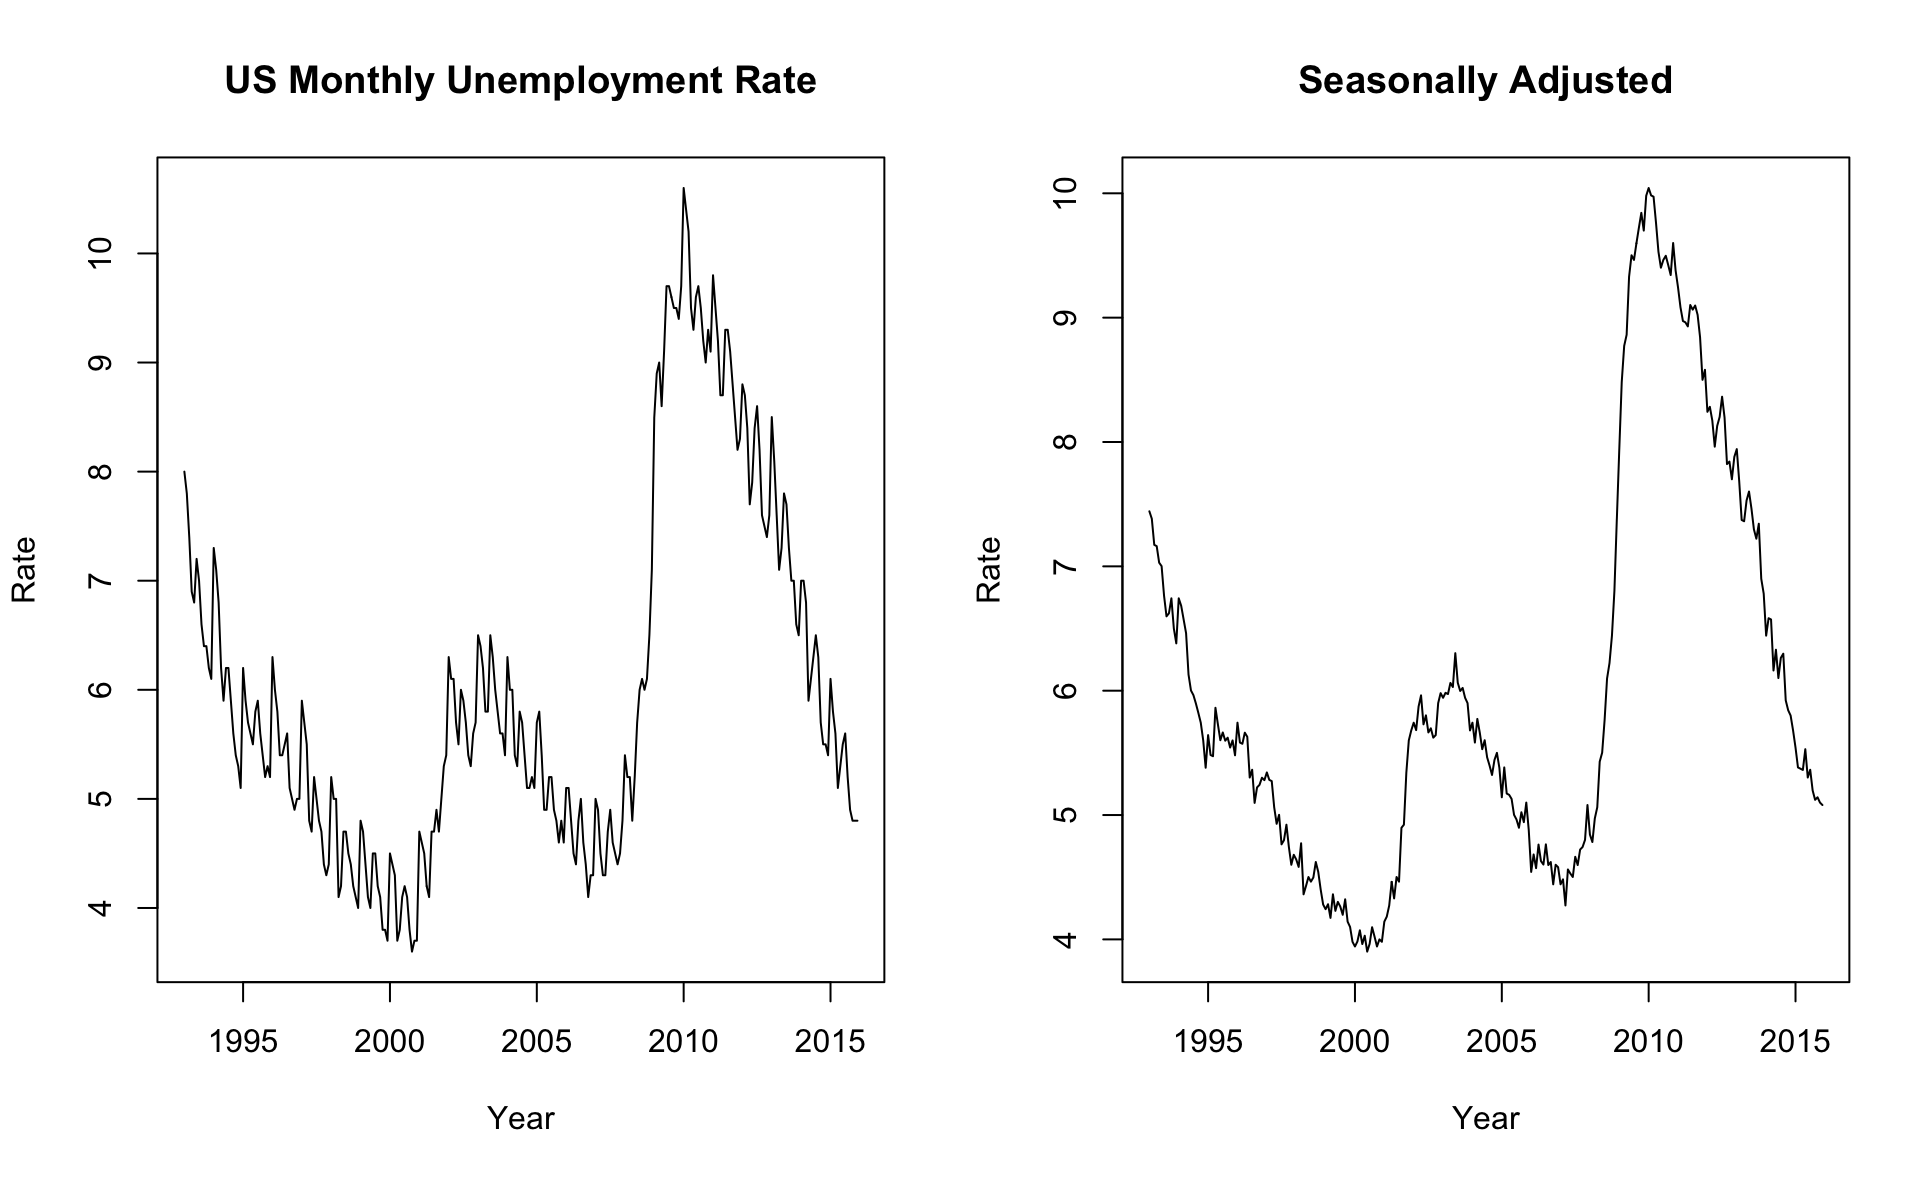
\includegraphics[width=.7\textwidth]{images/Unemployment}
		\end{figure}
		
		\subsection*{Stationarity}
						
			After the initial exploration of the time series graphs, the team has chosen to focus on building priliminary models which will serve as the foundation of further analysis. In looking at the inital plots, it appears that the series could benefit from detrending. As such, one of the primary goals has been to transform the data to stationarity. \newline
			
			An Augmented Dickey-Fuller (ADF) test for stationarity was conducted to verify the nonstationarity of the unemployment data.  The ADF test tests the null hypothesis that the time series data has a unit root against the alternative that the data are stationary \citep{shumway2010time}. For the non-seasonlly adjusted data the Dickey-Fuller test statistic was -1.4266, a lag order of 6, and a p-value of 0.8176. Additionally, the seasonally adjusted data had a Dickey-Fuller test statistic of -2.1377, a lag order of 6, and a p-value of 0.518. The high p-values suggest that we do not have a stationary model with just the raw unemployment data, whether or not the data are seasonally adjusted.\newline
			
			Taking the first and second differences resulted in considerably improved models.

		
 \begin{figure}[H]
      	\centering
      	\caption{Second differences with and without seasonal adjustments}
      	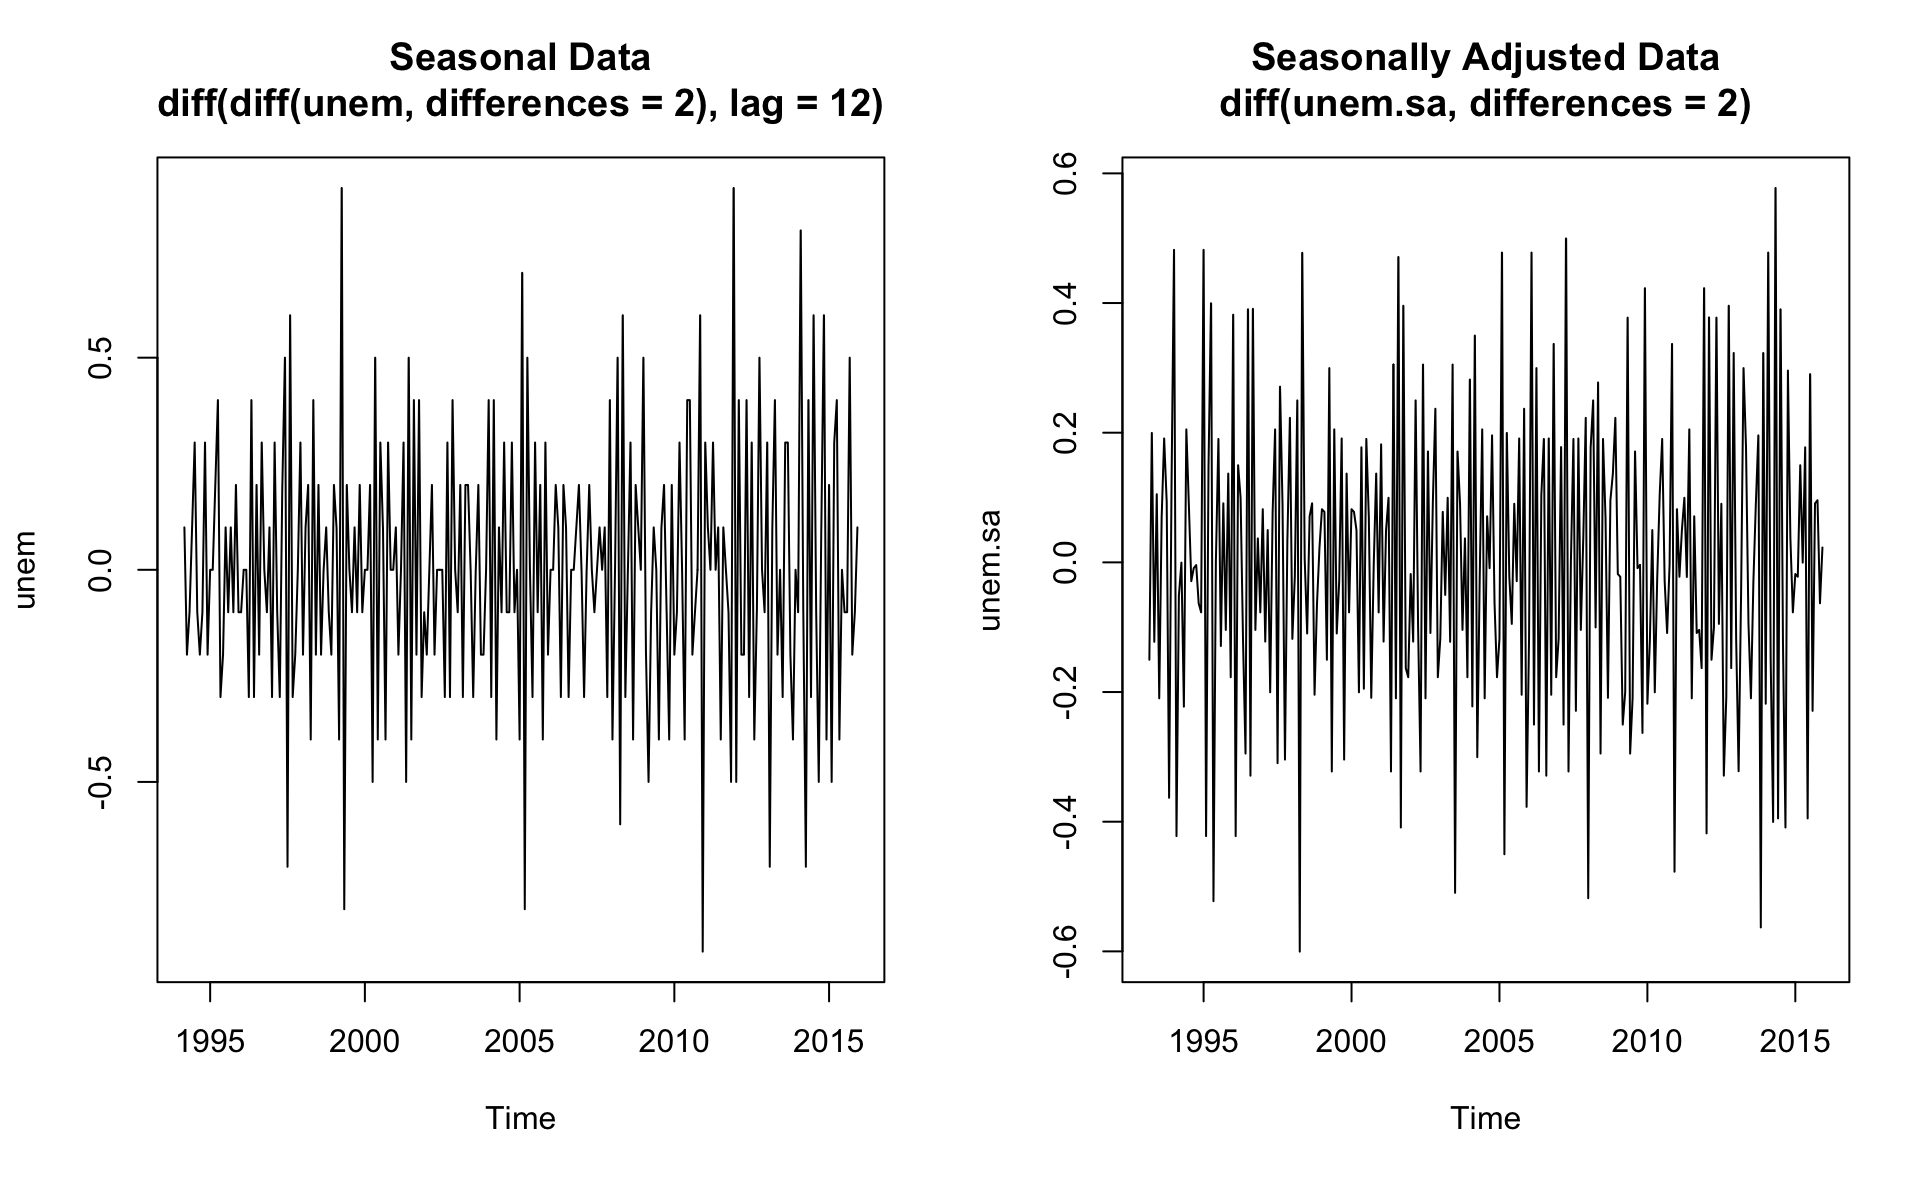
\includegraphics[width=.7\linewidth]{images/stationarity}
      	\label{fig:secdiff}
      \end{figure}
		
		%-----------------------------------------------------------------------------------------
		
		
		
		We just have unemployment data against second differences.
		Nothing too out of the ordinary.
		
		We see that lag 1 sticks outside the confidence band.  AR(1)
		Tailing off for seasonally adjusted.
		
		Shout out to the 3: Similar structure.
		detrended regressors.
		
		Just from the table AIC and BIC - Model 5 best bet.  But best may be something different.
		
		\begin{enumerate}
			\item 1st SARIMA model, second differences, moving average of order 12.
			Still working with lag 12 because as you remember from our last presentation the data was collected monthly.
			Residuals do look pretty good - nice and randomly distributed. 
			Huge drop with the recession of 2008, like initial unemployment plots see sharp drop.
			ACF inside the blue - residuals do not depend on each other.
			\item 2nd SARIMA model, 
			now we just the up the autoregression parts working with 1, 2, and 3 steps back.  
			Normally distributed residuals and do not depend on each other.
			\item  Similar to others except:
			only the AR part in the 1st part changed, now we are working with an autoregressive of order 4.
			4 steps but pictures do not look any different very good models.
			\item  Sharp drop in residuals around 2008
			\item Sean's favorite based on AIC and BIC alone. 
			residuals uncorrelated
			\item one acf barely sticking out
			\item same story - act stay in better
		\end{enumerate}
		
		question: p-values for Box statistic.... fall below band of 5\% how to interpret. Forget how to answer this question. What else can we garner. How can use for model selection.
		
		Of course, this month's unemployment will impact the next months. Not going to toss out the idea that all of the residuals are independent of each other. That may affect our forecasting in the future.
		
		Models 1, 2, \&3. Some are dipping below some hovering below.  One pokes out.  May be missing things that are going on.  Investigate.  Maybe at this lag something is happening with the residuals. We may need to look more closely.
		
		Personal opinion.  Favorite is number 5.  Best model based upon what we know now.
		
		Right... I do not recall which commands were used to generate these. See what was done. May be how the package was constructed.


			
			\begin{multicols}{2}
						I then plotted the first difference, and it appears relatively stationary.
						
							This is confirmed by the ADF test on the first differenced data, which has a very small p-value:
						
						Augmented Dickey-Fuller Test
						Dickey-Fuller = -4.3501, Lag order = 6, p-value = 0.01
						alternative hypothesis: stationary
						
						\begin{figure}[H]
							\centering
							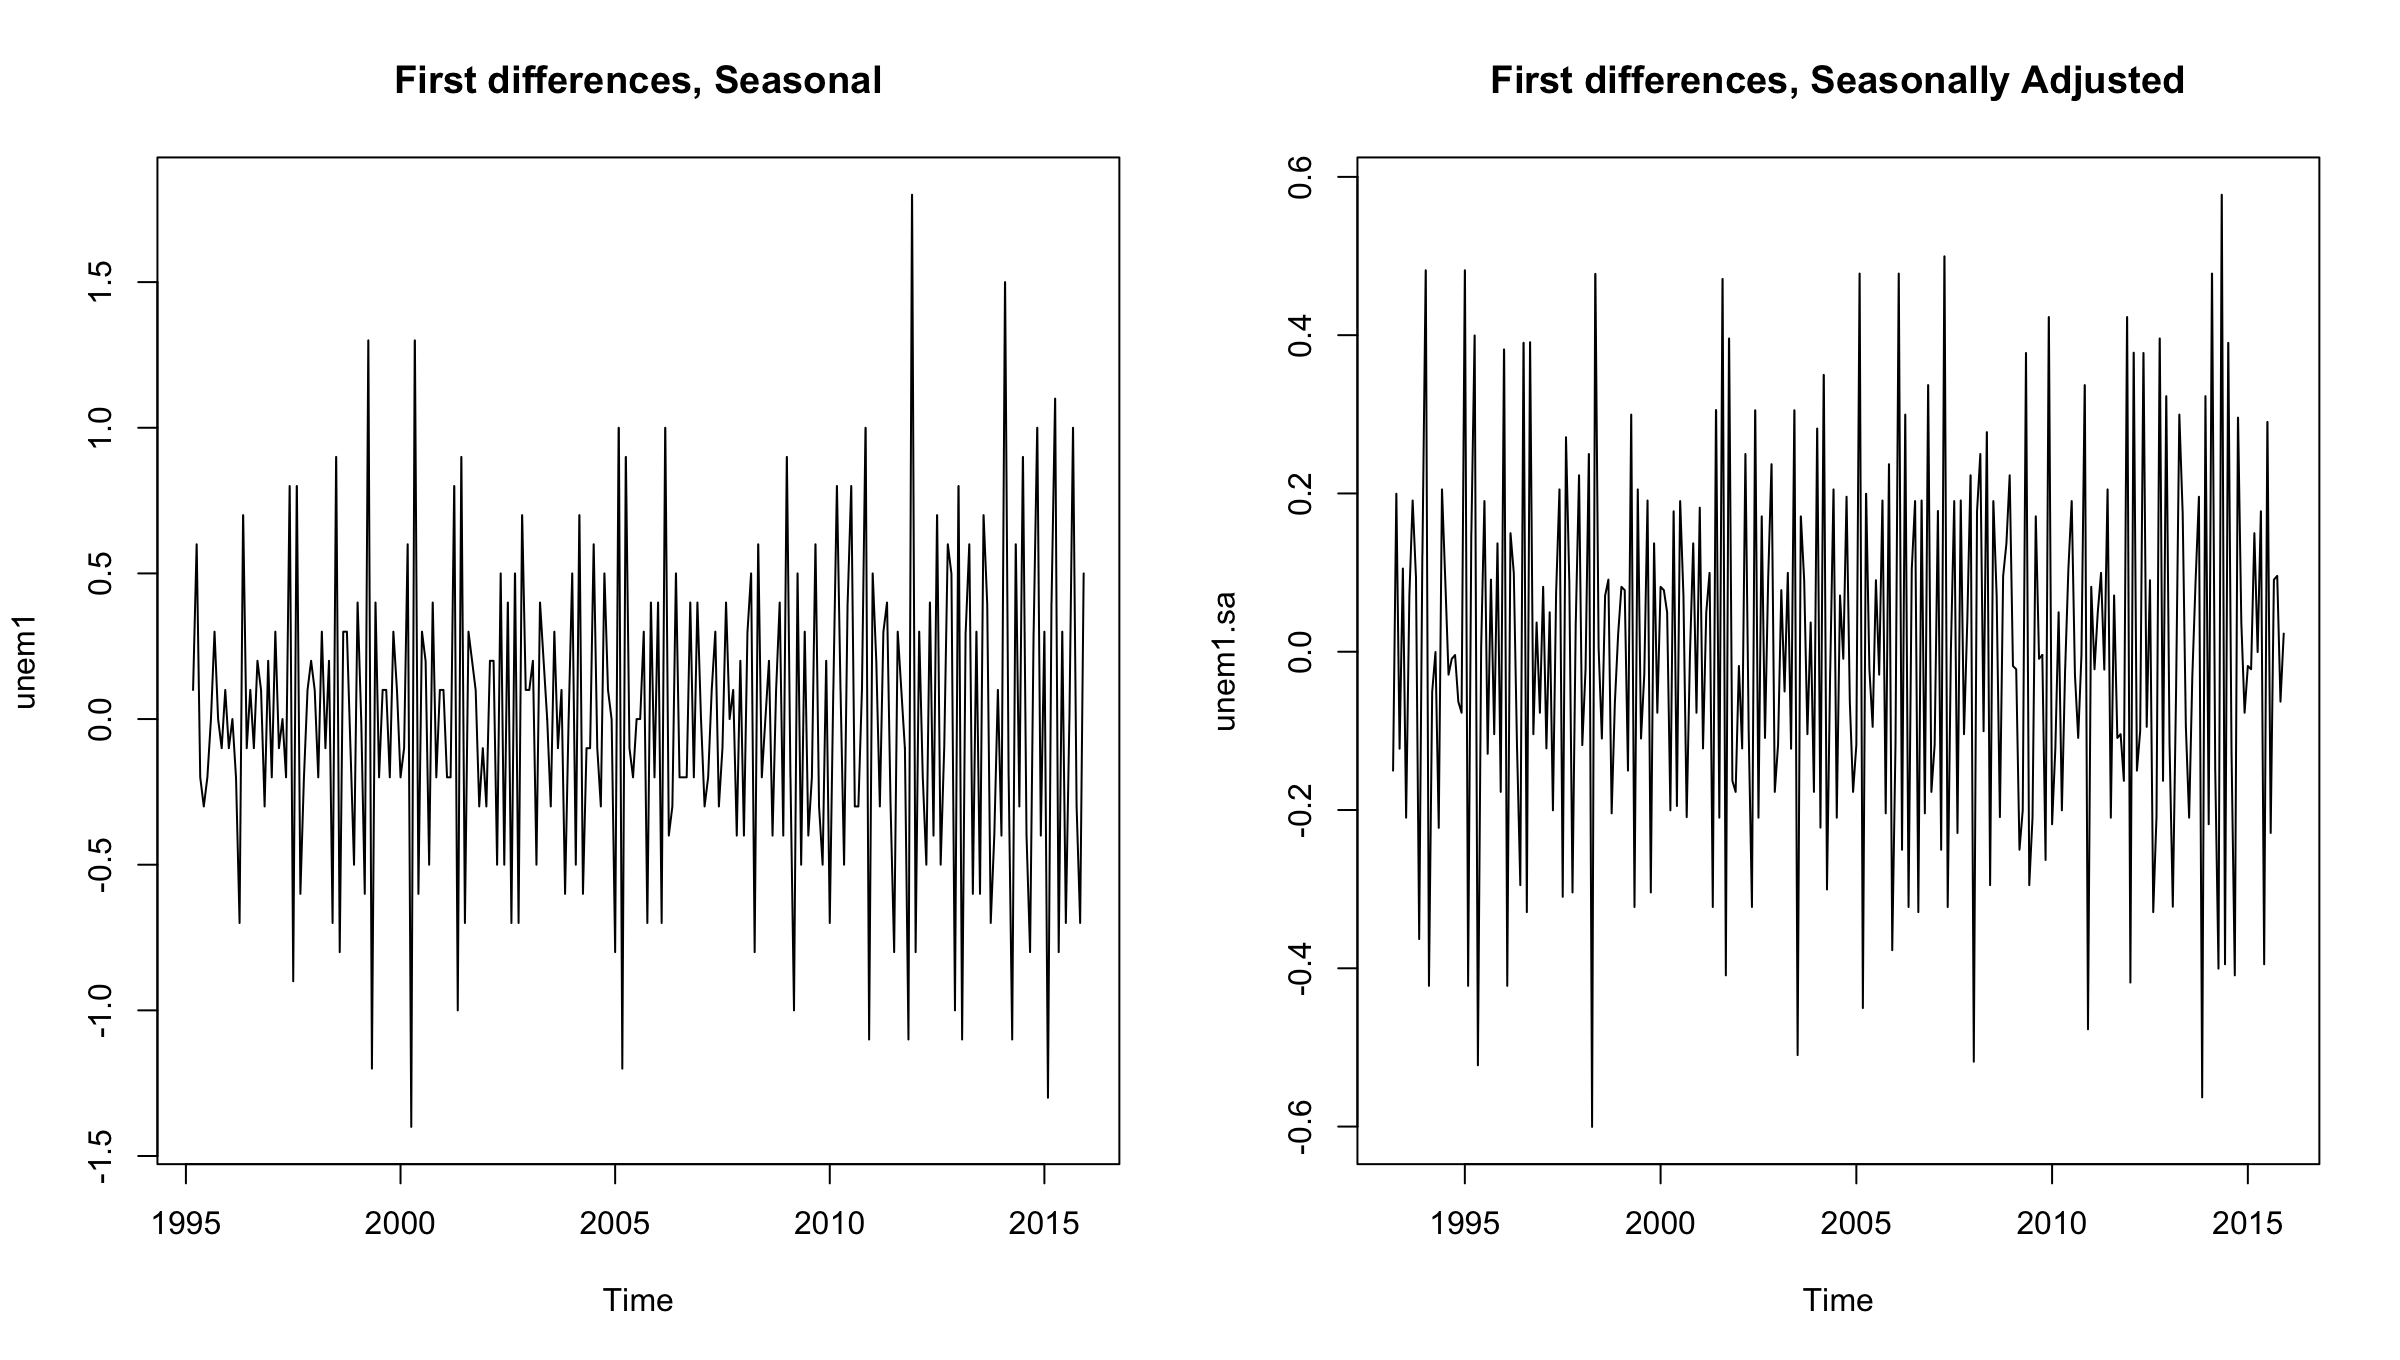
\includegraphics[width=.6\linewidth]{images/firstdiff}
							\caption{Plot of first Difference}
							\label{fig:firstdiff}
						\end{figure}
			\end{multicols}

	




%-----------------------------------------------------------------------------------------
  \subsection*{Differencing}
  
\begin{itemize}
	\item I took the second difference (d = 2), as Joseph suggested, then the first seasonal difference (D = 1) with s = 12 (this is common for monthly economic data), as the book did.
      
    \item   Below, Figure \ref{fig:secdiff},  is the plot of the transformed graphed. It looks pretty stationary (not perfect, but adequate), and we can confirm this with the ADF test (it's cited in other time series texts, but I haven't seen it in ours yet).
\end{itemize}
      
      \textit{I like the idea of using the ADF. We can include it as part of our literature review.}
      
      
     
  

%-----------------------------------------------------------------------------------------
  
  \subsection*{ACF \& PACF}
  \begin{itemize}
  	\item  After that, the book suggests that you examine the ACF and PACF plots.
  	 \item First, the book says to look at the seasonal changes in ACF and PACF (h = 12, 24, 36, ...). These seem to indicate that the ACF trails off, and the PACF cuts off after one year (h = 12). This suggests that we let P = 1 and Q = 0.
  	 \item Next, the book says to look at the ACF and PACF within only the first season (h = 1, 2, ..., 12). The PACF declines slowly, but the ACF cuts off after 1, suggesting we let p = 0, and q = 1.
  \end{itemize}
  
  



      \begin{figure}[H]
      	\centering
      	\caption{ACF \& PACF Plots}
      	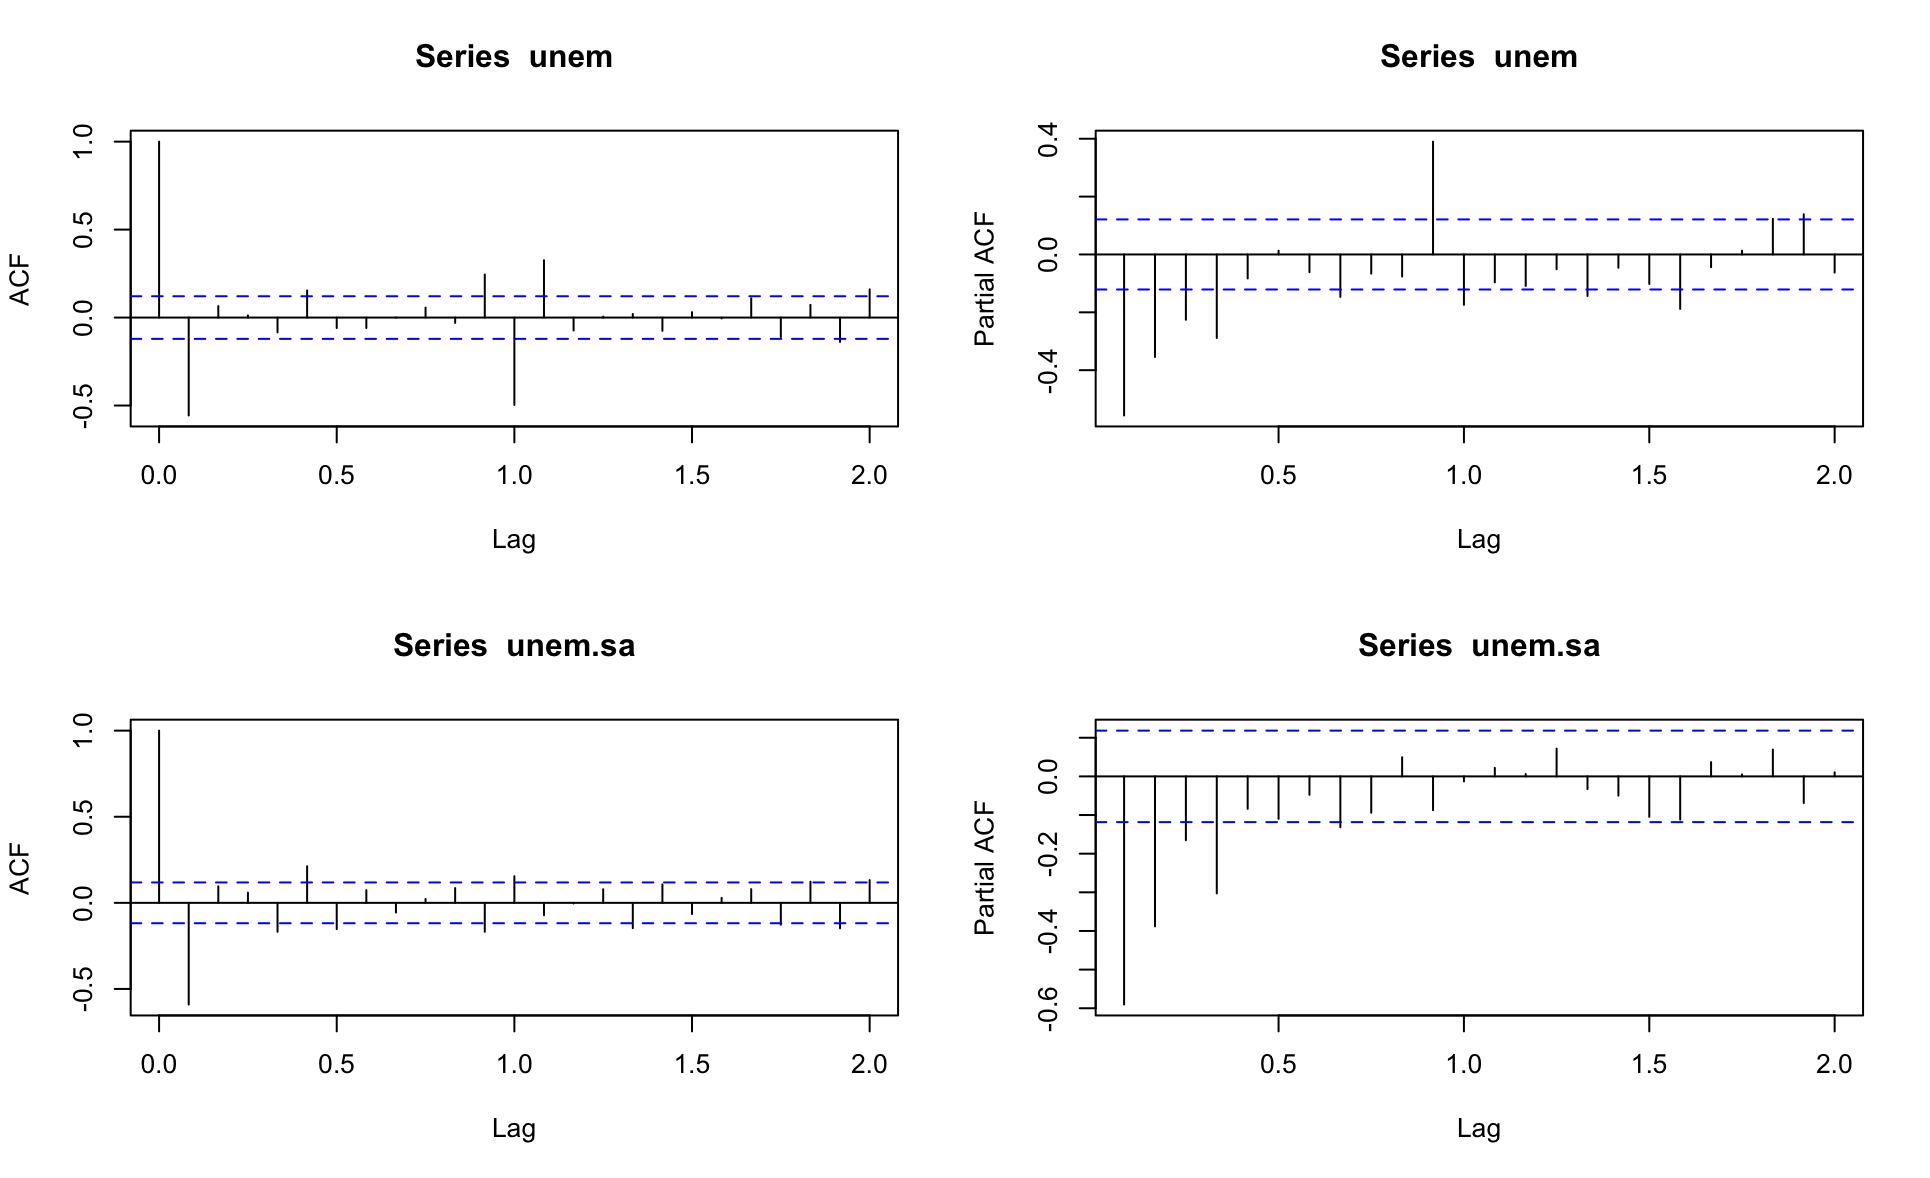
\includegraphics[width=\linewidth]{images/acfpacf}
      	\label{fig:secdiff2}
      \end{figure}
%----------------------------------------------------------------------------------------- 

    \section*{Model Comparisons}
    
\begin{itemize}
	\item     I then look at the ACF and PACF plots to build models. First, we can look into the seasonal pattern. The ACF seems to tail off and the PACF cuts off at either 1 or 3. Together, the plots suggest AR(1) or AR (3).

\item We then can inspect the plots at the within season lags, h=1,..,11. One perspective is that the ACF cuts off after 1 and the PACF tails off, and it indicates MA(1). Another perspective is that the ACF cuts off after 1 and the PACF cuts off after 4. In this situation, the book suggests to build a SARMA of orders p = 4 and q = 1. However, our professor points out that this is a bad reasoning. It is still however tempting for me to try this model since I lean to the side that the PACF cuts off after lag 4 instead of tails off (some subjective feeling goes in here). We right now don't know how to handle the situation where both ACF and PACF cuts off at a certain lag other than the approach mentioned in the book. So I tried this model. In diagnostic procedures, as you will see, it works better at some criterion. Together, I proposed two additional models and compare them to the one proposed by Travis.

 \item  From looking at AIC and BIC values, Models 2 and 3 perform quite similarly, which both show some slight evidence of outperforming Model1.
  
  \item Then we could compare the three models based on diagnostic plots. The standardized residuals of all models show some evidence of non-white-noise. ARMA models do not model variability. We will have a few lectures on this topic. There is not much we can do now on this issue.
  
 \item  In the ACF of residuals of Model 1 shows a spike at lag 24. The other two models do not show such a spike.
  
  \item The normal plots from the three models are fairly similar.
  
  \item The Q-statistic or Ljung-Box statistic:
  
  Models 1 and 2 have similar results. Model 1 seems to perform better at the first few lags, but Model 2 does better after lag 15. Model 3 clearly perform better than the two models on the Q-statistic. Since the Model 3 is based on a reasoning our professor does not like, we may not present this model. However it at least informs us that some models based on the thought that both the ACF and PACF cuts off at certain lags might model our data better. 
  
 \item  While going through a bunch of models, the following model seems most appropriate as noted by everyone. sarima(econ[,2],0,2,1,1,1,0,12) with the following diagnostics: [image: Inline image 2] The adf test also suggests stationarity as follows:  Also, I am working on other predictor variables to develop a preliminary regression model.
  
 \item  I am trying to fit the regression model here and was wondering if I should
take the stationary data for my fitting? Any help on this would be
appreciated.

\item I believe you would need to use the stationary non-seasonal unemployment rate as your response variable. I do not believe your predictor variables have to be stationary, but it would probably make sense to at least take the seasonality out of them.

\item Checking both residual plots shows that there is a drastic drop that is likely indicative of the 2008 recession. Can we add weighting or something to fix this?

\item In the political dataset I have an indicator variable for recession by month we could try using that. 

\item Regarding the expectations for presentation, the professor has not mentioned yet. However, in the last two lectures (14 and 15), he talked a lot applied examples about model building. I'd assume that our presentation would be something similar to what he talked in the two lectures. Basically, it's the model building process. How do we preprocess our data to obtain a stationary process (difference order 2 and difference order 1 in our case)? How do we identify the model (based on ACF and PACF)? What is the set of candidate models? How do you choose the best one (AIC, BIC, diagnostics)? I guess we might not need to present a regression model at this stage since he hasn't talked much about it. How do you guys think about this?

\item "Best model," as far as I know, is pretty ambiguous right now. With what I have done before, I checked AIC and BIC (not really thinking about using R-squared for the time being). The model identification from P/ACF is outlined in the text by checking out the tail behavior to see if it decays asymptotically or cuts off. We should be checking inside the band for "cutoff" behavior.

\item Sure, it's always hard to call a model "Best". I think in presentations, we may present several potential candidate models, and compare them from several perspectives. Hopefully, one model will gain relatively more evidence.

\item I would like to propose an additional model. I have gone through the same exercise as @trlilley12 and @bopangpsy only I used the seasonally adjusted unemployment rate. It looks like the performance is definitely comparable to the seasonal models. I used sarima for the nice diagnostic plot it creates, but I left the seasonal parameters out.

\end{itemize}

I get an AICc \(= -2.617631\) and BIC \(= -3.598962\)


mdl4 = sarima(xdata = unem, p = 1, d = 2, q = 1)

Call:
stats::arima(x = xdata, order = c(p, d, q), seasonal = list(order = c(P, D, 
Q), period = S), include.mean = !no.constant, optim.control = list(trace = trc, 
REPORT = 1, reltol = tol))

Coefficients:
ar1      ma1
-0.2021  -0.8078
s.e.   0.0688   0.0433

sigma\(^2\) estimated as 0.02626:  log likelihood = 109.15,  aic = -212.3

\$AIC
[1] -2.625197

\$AICc
[1] -2.617631

\$BIC
[1] -3.598962


Cool, Joseph! This model is simple and performs pretty well in terms of both fitting indices and diagnostics.
%--------------------------------------------------------------------------------------------------------------------------------------------------------------------------------------	

\bibliographystyle{plainnat} % or try abbrvnat or unsrtnat
\begin{flushleft}
\bibliography{main} % refers to example.bib
\end{flushleft}
}
  

\end{document}